% Created 2020-04-10 Fri 21:52
% Intended LaTeX compiler: pdflatex
\documentclass[11pt]{article}
\usepackage[utf8]{inputenc}
\usepackage[T1]{fontenc}
\usepackage{graphicx}
\usepackage{grffile}
\usepackage{longtable}
\usepackage{wrapfig}
\usepackage{rotating}
\usepackage[normalem]{ulem}
\usepackage{amsmath}
\usepackage{textcomp}
\usepackage{amssymb}
\usepackage{capt-of}
\usepackage{hyperref}
\usepackage{minted}
\usepackage[margin=0.75in]{geometry}
\author{Tigany Zarrouk}
\date{\today}
\title{Final Ti Model Results}
\hypersetup{
 pdfauthor={Tigany Zarrouk},
 pdftitle={Final Ti Model Results},
 pdfkeywords={},
 pdfsubject={},
 pdfcreator={Emacs 26.3 (Org mode 9.1.9)}, 
 pdflang={English}}
\begin{document}

\maketitle
\tableofcontents


\section{Objective Function}
\label{sec:org93a8fbb}



PARAMETERS
  fdd=0.1958363809 qdds=0.5591275855 qddp=0.5690351902 qddd=0.7745947522 b0=58.0906936439 p0=1.2185323579 b1=-3.2299188646 p1=0.6862915307 b2=593519.1134129359 m2=-11.5000000000 p2=0.0000000000 ndt=2.0000000000 cr1=-6.0000000000 cr2=3.0474400934 cr3=-1.2317472193 r1dd=6.5000000000 rcdd=10.0000000000 rmaxhm=10.1000000000 npar=18 
VARGS
    -vfdd=0.1958363809 -vqdds=0.5591275855 -vqddp=0.5690351902 -vqddd=0.7745947522 -vb0=58.0906936439 -vp0=1.2185323579 -vb1=-3.2299188646 -vp1=0.6862915307 -vb2=593519.1134129359 -vm2=-11.5000000000 -vp2=0.0000000000 -vndt=2.0000000000 -vcr1=-6.0000000000 -vcr2=3.0474400934 -vcr3=-1.2317472193 -vr1dd=6.5000000000 -vrcdd=10.0000000000 -vrmaxhm=10.1000000000 



\begin{center}
\begin{tabular}{lrr}
Quantity & From Model & Target\\
\hline
a\(_{\text{hcp}}\) & 5.58523112 & 5.57678969\\
c/a & 1.58371266 & 1.58731122\\
a\(_{\text{omega}}\) & 8.93475285 & 8.73254342\\
c\(_{\text{omega}}\) & 5.38726911 & 5.32343103\\
a\(_{\text{4h}}\) & 5.57584691 & 5.56325146\\
c\(_{\text{4h}}\) & 18.09810672 & 17.75908031\\
a\(_{\text{6h}}\) & 5.57365569 & 5.54639384\\
c\(_{\text{6h}}\) & 27.18378460 & 26.77136353\\
a\(_{\text{bcc}}\) & 6.20079768 & 6.17948863\\
a\(_{\text{fcc}}\) & 7.87290654 & 7.88677000\\
DE(o,h) & 0.58764167 & -0.63343333\\
DE(4h,h) & 1.58019500 & 3.17160000\\
DE(6h,h) & 2.48264833 & 3.72005000\\
DE(b,h) & 5.35128500 & 7.63520000\\
DE(f,h) & 3.78088500 & 4.51880000\\
c\(_{\text{11}}\) & 171.60928873 & 176.10000000\\
c\(_{\text{33}}\) & 198.90063708 & 190.50000000\\
c\(_{\text{44}}\) & 47.42549704 & 50.80000000\\
c\(_{\text{12}}\) & 94.65941969 & 86.90000000\\
c\(_{\text{13}}\) & 61.22624060 & 68.30000000\\
M\(_{\text{freq}}\)\(_{\text{0}}\) & 2.59341377 & 2.85858719\\
M\(_{\text{freq}}\)\(_{\text{1}}\) & 2.59341378 & 2.85858719\\
M\(_{\text{freq}}\)\(_{\text{2}}\) & 2.59341378 & 2.85858719\\
M\(_{\text{freq}}\)\(_{\text{3}}\) & 2.59341379 & 2.85858719\\
M\(_{\text{freq}}\)\(_{\text{4}}\) & 5.85272461 & 5.66706047\\
M\(_{\text{freq}}\)\(_{\text{5}}\) & 5.85272461 & 5.66706047\\
H\(_{\text{freq}}\)\(_{\text{0}}\) & 3.82320403 & 4.80643423\\
H\(_{\text{freq}}\)\(_{\text{1}}\) & 3.82320403 & 5.58010025\\
H\(_{\text{freq}}\)\(_{\text{2}}\) & 6.40288977 & 5.65316738\\
H\(_{\text{freq}}\)\(_{\text{3}}\) & 6.40288977 & 6.36651842\\
H\(_{\text{freq}}\)\(_{\text{4}}\) & 7.92857431 & 6.40050186\\
H\(_{\text{freq}}\)\(_{\text{5}}\) & 7.92857431 & 7.64082373\\
bandw.  G & 3.69394702 & 5.87085872\\
bandw.  K & 4.65178817 & 4.97424321\\
bandw.  M & 5.19329495 & 7.78109872\\
bandw.  L & 4.21232412 & 6.34433701\\
bandw.  H & 3.54700549 & 9.70902614\\
DOSerr\(_{\text{h}}\) & 0.00000000 & 0.00000000\\
DOSerr\(_{\text{o}}\) & 0.00000000 & 0.00000000\\
E\(_{\text{pris}}\)\(_{\text{f}}\) & 98.95340236 & 220.00000000\\
\end{tabular}
\end{center}



----------     E\(_{\text{prismatic}}\)\(_{\text{fault}}\)     -----------

\begin{center}
\begin{tabular}{lrll}
tbe: & 98.953 & mJ/m\(^{\text{2}}\) & \\
DFT: & 250.000 & mJ/m\(^{\text{2}}\) & [Benoit  2012]\\
DFT: & 233.000 & mJ/m\(^{\text{2}}\) & [Ackland 1999]\\
\end{tabular}
\end{center}


----------     E\(_{\text{Basal}}\)\(_{\text{fault}}\) I2     -----------

\begin{center}
\begin{tabular}{lrll}
tbe: & 211.658 & mJ/m\(^{\text{2}}\) & \\
DFT: & 260.000 & mJ/m\(^{\text{2}}\) & [Benoit  2012]\\
\end{tabular}
\end{center}


\section{Phonons}
\label{sec:org2210cda}

\subsection{Harmonic}
\label{sec:org9565b19}

\subsection{Quasiharmonic Effects}
\label{sec:org658828b}

\subsubsection{Gibbs free energy}
\label{sec:orgd1ff7e7}

\begin{center}
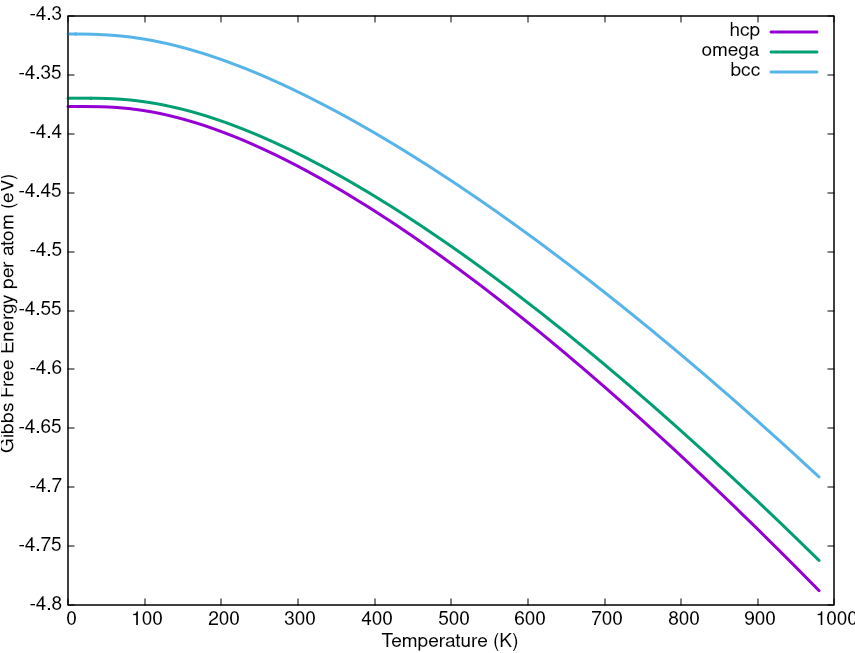
\includegraphics[width=.9\linewidth]{Images/gibbs_free_energy_per_atom_2020-04-02.png}
\end{center}
\begin{center}
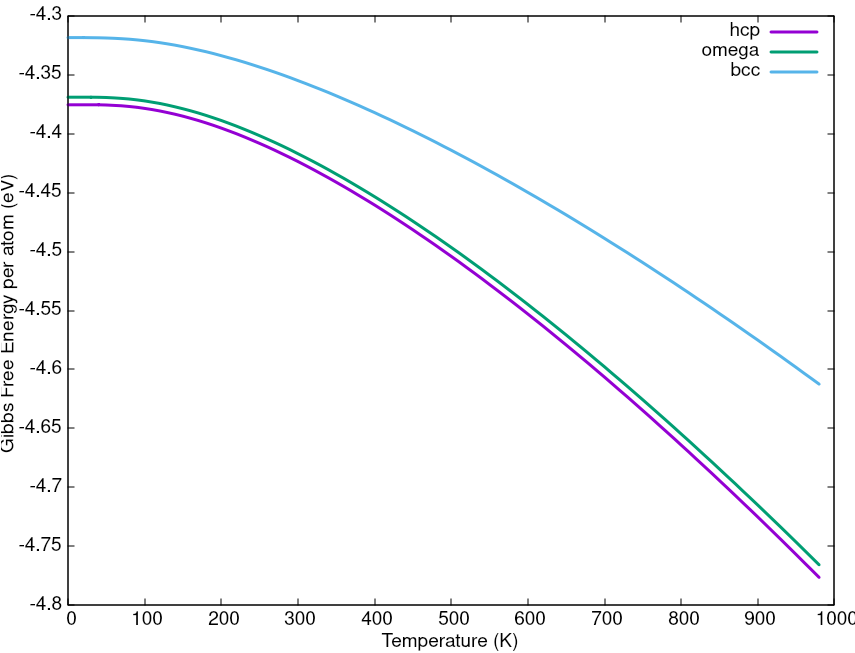
\includegraphics[width=.9\linewidth]{Images/gibbs_free_energy_per_atom_2020-04-02_4x4x4.png}
\end{center}



\subsubsection{Thermal Expansion}
\label{sec:org1c4b190}

This is roughly four times higher than one would expect from
experiment. 
\begin{center}
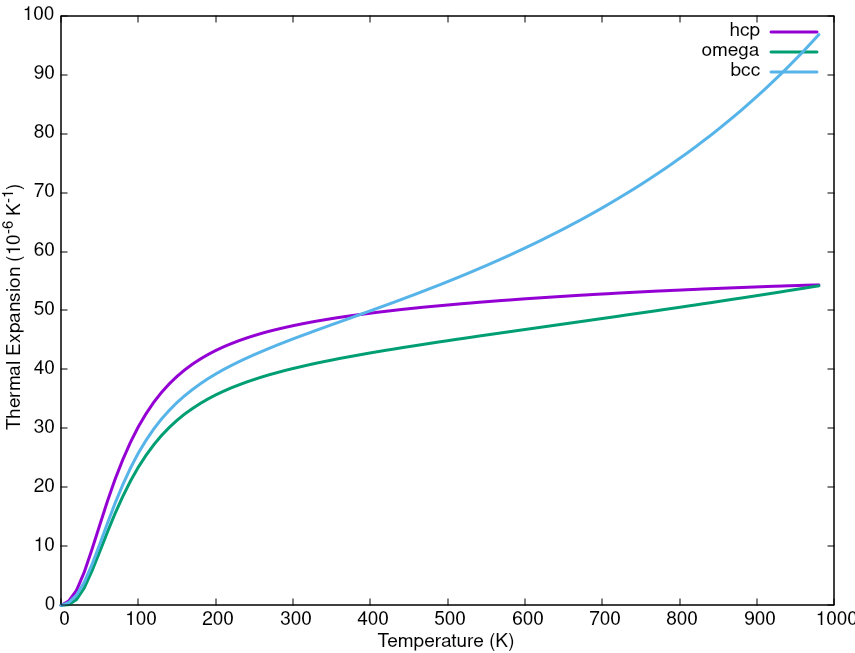
\includegraphics[width=.9\linewidth]{Images/thermal_expansion_all_phases_2020-04-02.png}
\end{center}

\begin{center}
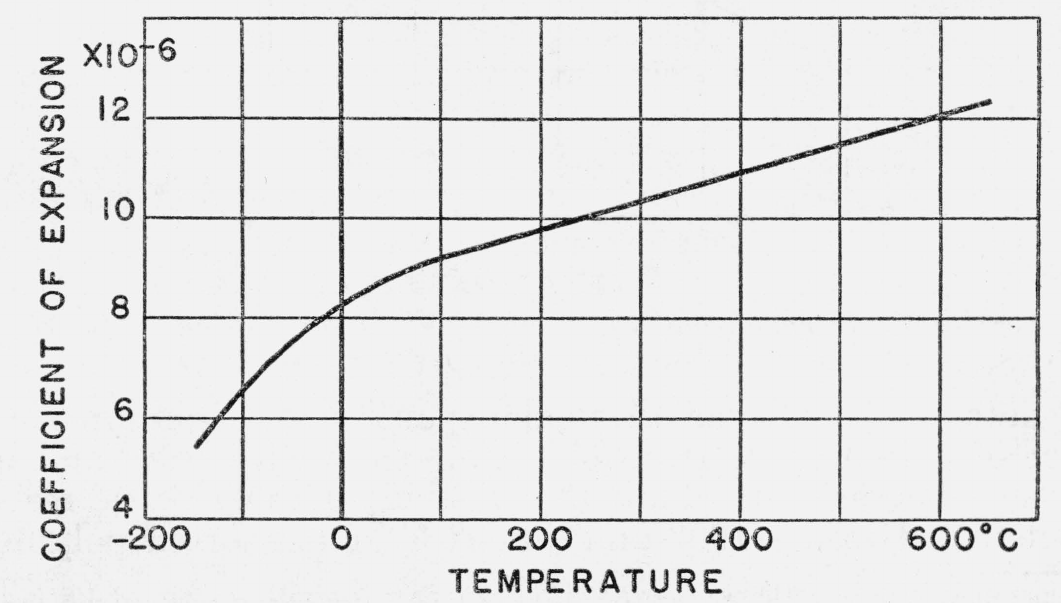
\includegraphics[width=.9\linewidth]{Images/thermal_expansion_alpha_ti_exp.png}
\end{center}

\section{Defect Clusters}
\label{sec:org41041a6}

----------     E\(_{\text{vacancy}}\)\(_{\text{formation}}\)     ----------

\begin{center}
\begin{tabular}{lll}
tbe: & 2.347  eV & \\
DFT: & 1.950  eV & GGA-PAW:   Angsten  (2013)\\
exp: & 1.270  eV & Hashimoto  (1984)\\
\end{tabular}
\end{center}

\subsection{Octahedral O interstitial relaxation}
\label{sec:org40d2f23}

Initial:
\begin{center}
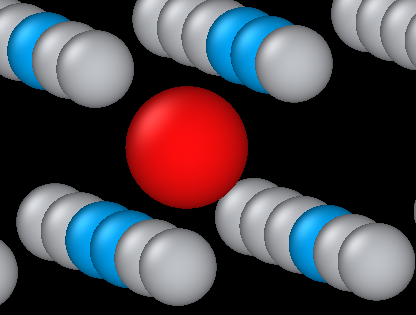
\includegraphics[width=.9\linewidth]{Images/initial_octahedral_ox_ovito.png}
\end{center}

Final:
\begin{center}
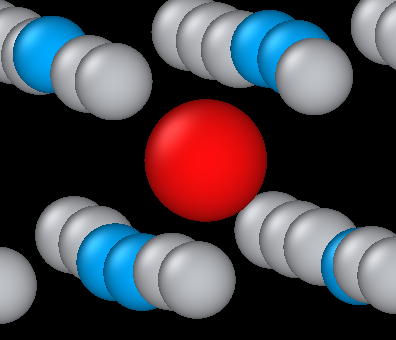
\includegraphics[width=.9\linewidth]{Images/final_octahedral_ox_ovito.png}
\end{center}

\subsection{Tetrahedral O interstitial relaxation}
\label{sec:org0810611}

Initial:
\begin{center}
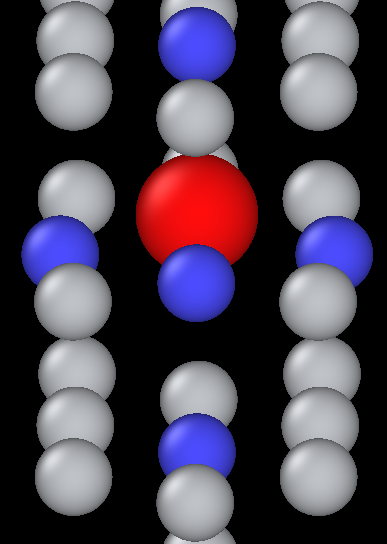
\includegraphics[width=.9\linewidth]{Images/final_model_final_tetra_ox.png}
\end{center}

Final:
\begin{center}
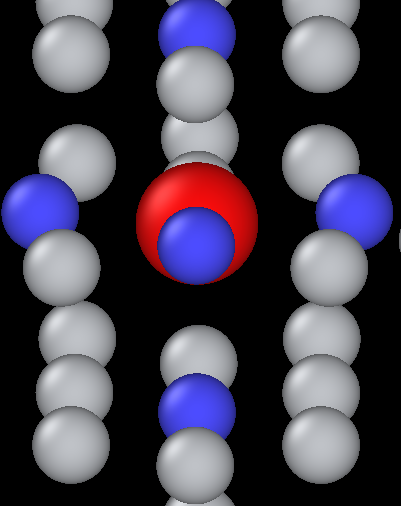
\includegraphics[width=.9\linewidth]{Images/final_model_initial_tetra_ox_ovito.png}
\end{center}

\subsection{Energies for defects}
\label{sec:orgfa89c8e}

Relative differences are 

>> (E\(_{\text{tetrahedral}}\) - E\(_{\text{octahedral}}\)) 
\begin{center}
\begin{tabular}{lll}
tbe: & 1.65 eV & \\
GGA-DFT: & 1.23 eV & Kwasniak (2013)\\
\end{tabular}
\end{center}

>> (E\(_{\text{hexahedral}}\) - E\(_{\text{octahedral}}\))
\begin{center}
\begin{tabular}{ll}
tbe: & 0.90 eV\\
\end{tabular}
\end{center}

> Note: Preference for tetrahedral oxygen to go into hexahedral site as seen by images above

All formation energies below use the chemical potential of Akysonov
(2013) of value \(\mu_{\text{oxygen}} = \frac{5.6}{ 2} eV\).

\subsection{All formation energies}
\label{sec:org16c50f3}

\begin{center}
\begin{tabular}{ll}
Quantity & Energy (eV)\\
\hline
Ef\(_{\text{Vf}}\) & 2.347\\
 & \\
Ef\(_{\text{T}}\)\(_{\text{sol}}\) & -  21.783\\
Ef\(_{\text{O}}\)\(_{\text{sol}}\) & -  23.436\\
Ef\(_{\text{OO}}\)\(_{\text{sol}}\) & -  49.606\\
Ef\(_{\text{OOO}}\)\(_{\text{sol}}\) & -  76.037\\
Ef\(_{\text{OOOO}}\)\(_{\text{sol}}\) & - 102.470\\
Ef\(_{\text{OOOOO}}\)\(_{\text{sol}}\) & - 128.781\\
Ef\(_{\text{OOOOOO}}\)\(_{\text{sol}}\) & - 155.148\\
 & \\
Ef\(_{\text{T}}\)\(_{\text{dil}}\)\(_{\text{imp}}\) & -  28.991\\
Ef\(_{\text{O}}\)\(_{\text{dil}}\)\(_{\text{imp}}\) & -  30.645\\
Ef\(_{\text{OO}}\)\(_{\text{dil}}\)\(_{\text{imp}}\) & -  56.814\\
Ef\(_{\text{OOO}}\)\(_{\text{dil}}\)\(_{\text{imp}}\) & -  83.246\\
Ef\(_{\text{OOOO}}\)\(_{\text{dil}}\)\(_{\text{imp}}\) & - 109.679\\
Ef\(_{\text{OOOOO}}\)\(_{\text{dil}}\)\(_{\text{imp}}\) & - 135.989\\
Ef\(_{\text{OOOOOO}}\)\(_{\text{dil}}\)\(_{\text{imp}}\) & - 162.357\\
 & \\
Ef\(_{\text{T}}\)\(_{\text{formation}}\) & -  21.783\\
Ef\(_{\text{O}}\)\(_{\text{formation}}\) & -  23.436\\
Ef\(_{\text{OO}}\)\(_{\text{formation}}\) & -  46.806\\
Ef\(_{\text{OOO}}\)\(_{\text{formation}}\) & -  70.437\\
Ef\(_{\text{OOOO}}\)\(_{\text{formation}}\) & -  94.070\\
Ef\(_{\text{OOOOO}}\)\(_{\text{formation}}\) & - 117.581\\
Ef\(_{\text{OOOOOO}}\)\(_{\text{formation}}\) & - 141.148\\
 & \\
Ef\(_{\text{T}}\)\(_{\text{V}}\)\(_{\text{formation}}\) & -  18.905\\
Ef\(_{\text{O}}\)\(_{\text{V}}\)\(_{\text{formation}}\) & -  18.905\\
Ef\(_{\text{OO}}\)\(_{\text{V}}\)\(_{\text{formation}}\) & -  41.910\\
Ef\(_{\text{OOO}}\)\(_{\text{V}}\)\(_{\text{formation}}\) & -  66.013\\
Ef\(_{\text{OOOO}}\)\(_{\text{V}}\)\(_{\text{formation}}\) & -  88.998\\
Ef\(_{\text{OOOOO}}\)\(_{\text{V}}\)\(_{\text{formation}}\) & - 113.649\\
Ef\(_{\text{OOOOOO}}\)\(_{\text{V}}\)\(_{\text{formation}}\) & - 137.110\\
 & \\
Ef\(_{\text{T}}\)\(_{\text{vac}}\)\(_{\text{sol}}\)\(_{\text{bind}}\) & -   0.530\\
Ef\(_{\text{O}}\)\(_{\text{vac}}\)\(_{\text{sol}}\)\(_{\text{bind}}\) & -   2.183\\
Ef\(_{\text{OO}}\)\(_{\text{vac}}\)\(_{\text{sol}}\)\(_{\text{bind}}\) & -   2.547\\
Ef\(_{\text{OOO}}\)\(_{\text{vac}}\)\(_{\text{sol}}\)\(_{\text{bind}}\) & -   2.076\\
Ef\(_{\text{OOOO}}\)\(_{\text{vac}}\)\(_{\text{sol}}\)\(_{\text{bind}}\) & -  2.724\\
Ef\(_{\text{OOOOO}}\)\(_{\text{vac}}\)\(_{\text{sol}}\)\(_{\text{bind}}\) & - 1.583\\
Ef\(_{\text{OOOOOO}}\)\(_{\text{vac}}\)\(_{\text{sol}}\)\(_{\text{bind}}\) & - 1.690\\
\end{tabular}
\end{center}


\section{Binding energy of defect clusters in the harmonic approximation}
\label{sec:org66bacb5}

Using the defect cluster configurations mentioned earlier, one can
find the change in defect cluster formation free energies as a
function of temperature by using the harmonic approximation. 

To build the dynamical matrix, to obtain the vibrational free energy
contribution, one used phonopy to generate the displacements for nearest/next-nearest
neighbours to the defect, as the local atomic environment of atoms
past the second-nearest shells would have hardly changed from the
perfect lattice. From this vibrational frequencies were used to
obtain the full free energy of bindng of the defect as a function of
temperature. 


It would be interesting to see how the quasi-harmonic approximation
would change improve the accuracy of temperature/concentration
predictions with the addition of the change in the lattice parameter
with temperature. 

\section{Gamma surfaces}
\label{sec:org93e9e6c}

Energies are accurate to within 2 mJm\(^{\text{-2}}\), comparing the energies of
points in the corners which (the zeros of energy). So surface energies
might be \(\pm 2\) mJm\(^{\text{-2}}\) off which is reasonable. 

These calculations were done in tight binding with 15 layers for both
basal and prismatic. The k-points for the prismatic gamma surfaces were, and for basal they were. 
DFT comparisons are usind results of Rodney. 

The Pyramidal surface was obtained using the same 32 atom cell that
Ready used in his paper on the pyramidal gamma surface with DFT
pseudopotentials. 

\begin{center}
\begin{tabular}{ll}
Stacking Fault & Energy [mJm\(^{-2}\)]\\
\hline
Prismatic & \\
Basal \(I_2\) & \\
Basal & \\
Pyramidal I & \\
\end{tabular}
\end{center}

\newpage
\subsection{Basal}
\label{sec:org3fca5e0}

TBE:
\begin{center}
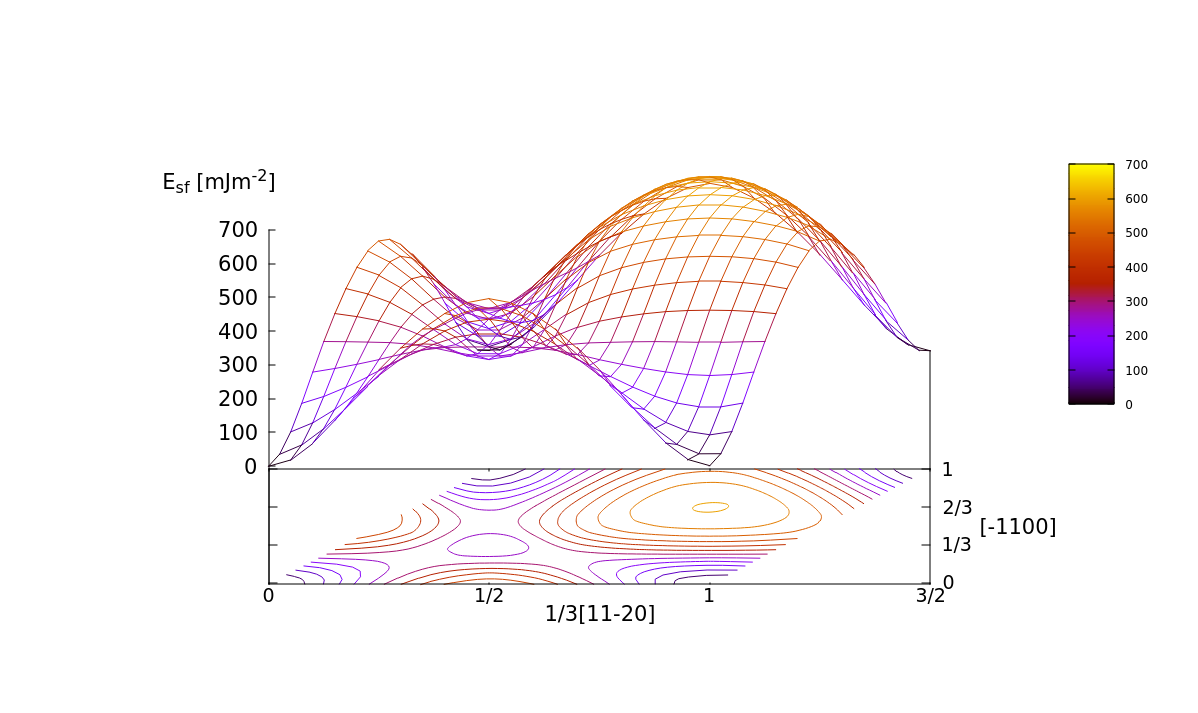
\includegraphics[width=.9\linewidth]{Images/basal_gamma_surface_final_model_2020-01-15.png}
\end{center}


DFT:
\begin{center}
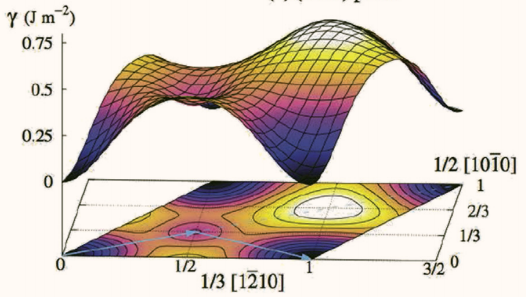
\includegraphics[width=.9\linewidth]{Images/rodney_basal_ti_gamma_surface.png}
\end{center}

\subsection{Prismatic}
\label{sec:org848dac6}

TBE:
\begin{center}
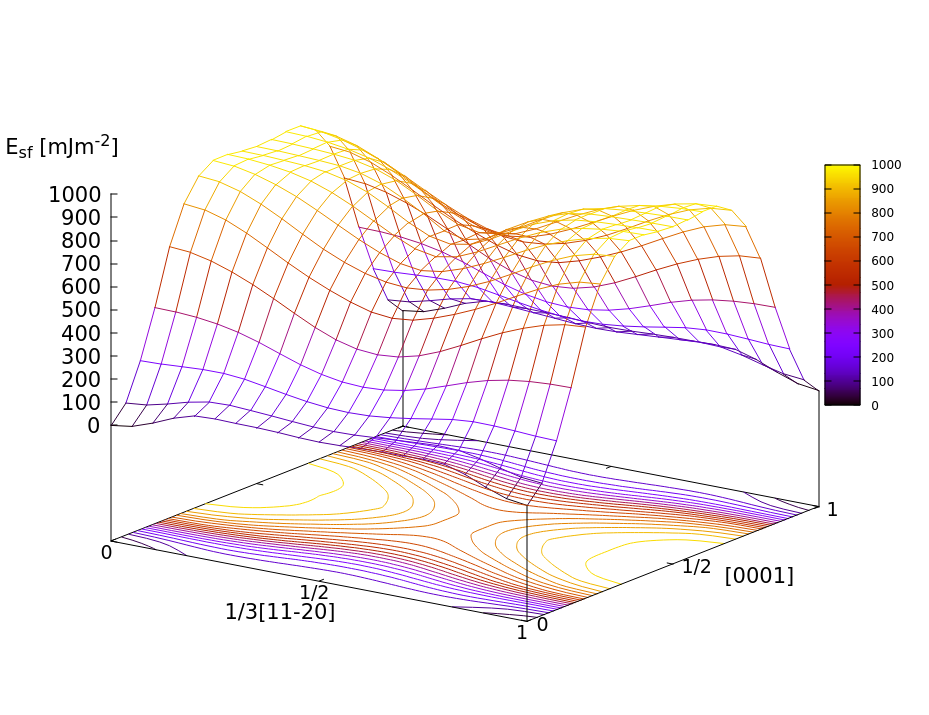
\includegraphics[width=.9\linewidth]{Images/prismatic_gamma_surface_final_model_angle_smaller.png}
\end{center}

DFT:
\begin{center}
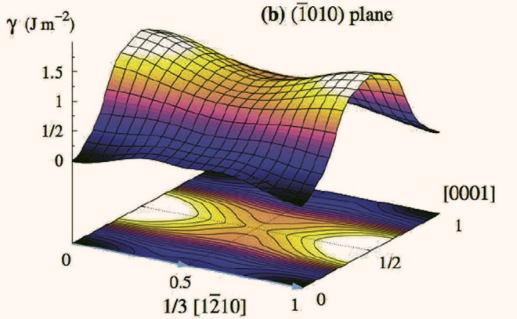
\includegraphics[width=.9\linewidth]{Images/rodney_prismatic_ti_gamma_surface.png}
\end{center}

\subsection{Pyramidal first order}
\label{sec:org2e25441}

TBE:
\begin{center}
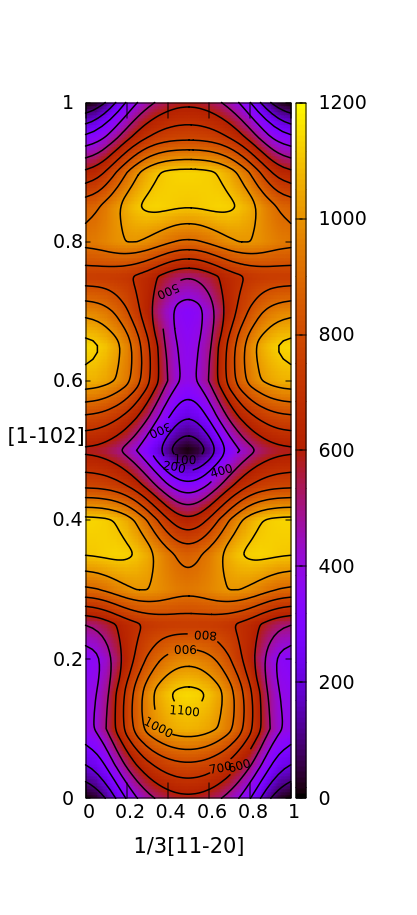
\includegraphics[width=.9\linewidth]{Images/pyramidal_gamma_surface_final_model_contours.png}
\end{center}
DFT pseudopot:
\begin{center}
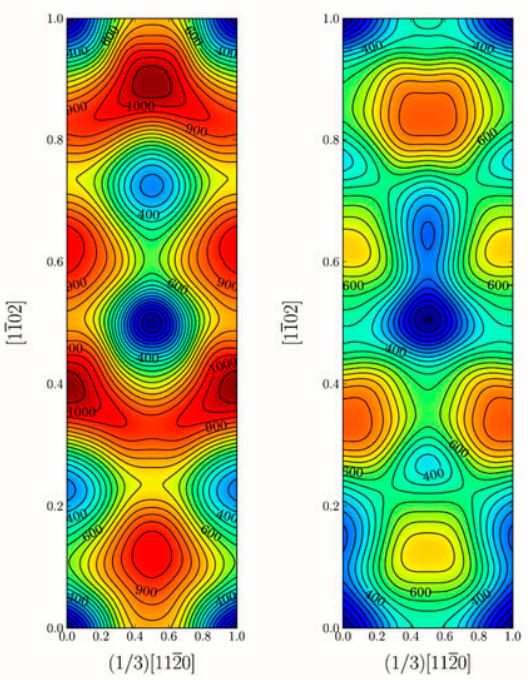
\includegraphics[width=.9\linewidth]{Images/pyramidal_gamma_surface_ready_data_both.png}
\end{center}

\subsection{Data}
\label{sec:org71fc201}
\href{file:///home/tigany/Documents/ti/final\_model\_2019-11-12/results\_2019-11-09\_muc/gamma\_surfaces/basal/basal\_gs\_noo\_alat\_energies.dat}{basal\(_{\text{gs}}\)\(_{\text{data}}\)}
\href{file:///home/tigany/Documents/ti/final\_model\_2019-11-12/results\_2019-11-09\_muc/gamma\_surfaces/prismatic/prismatic\_gs\_noo\_alat\_energies.dat}{prismatic\(_{\text{gs}}\)\(_{\text{data}}\)}
\href{file:///home/tigany/Documents/ti/final\_model\_2019-11-12/gamma\_surfaces/pyramidal\_results\_2019-11-13/pyramidal\_gamma\_surface\_2019-11-13.dat}{pyramidal\(_{\text{gs}}\)\(_{\text{data}}\)}
\section{Dislocation core structures}
\label{sec:orgc5874ef}


\subsection{Quadrupolar Array}
\label{sec:org5eb7d5c}

\subsubsection{Methodology}
\label{sec:orgdc2b6ba}
In the following, we see results of dislocation relaxation. The partial differential
displacement maps are of dislocations in their initial and final states in different initial
positions. The burger's vector seen in these plots is the partial \(1/6 [11\bar{2}0]\). The
original dislocation, of burger's vector \(1/3 [11\bar{2}0]\), should dissociate into two
dislocations on the primatic plane, each with burger's vector \(1/6 [11\bar{2}0]\). The atoms were
relaxed until the root-mean square force acting on each atom was less than \(4\times 10^{-5}\)
Ryd/Bohr.

These relaxations can be distinguished by the different initial
positions of the dislocation centre (elastic centre) as following
the paper by Tarrat \cite{Tarrat2009}. Cell geometry was 16x16x1,
where the unit cell was of four atoms, with \(x\), \(y\) and \(z\) axes
given by \([0001]\), \([\bar{1}100]\) and \(1/3[11\bar{2}0]\)
respectively. 

\begin{center}
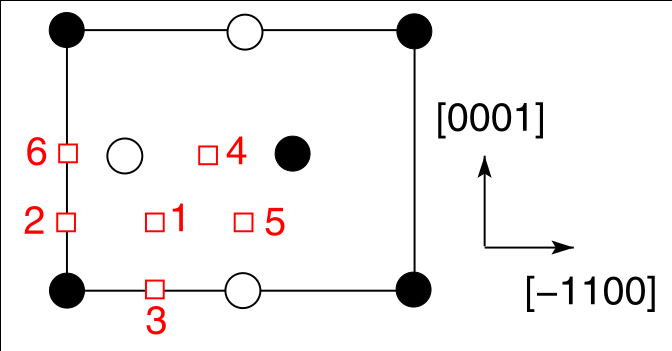
\includegraphics[width=.9\linewidth]{Images/tarrat_hcp_core_structures.png}
\end{center}

A quadrupolar array of dislocations was created using the "S"
arrangement of Clouet \cite{Clouet2012}: the cut plane of the
dislocation dipole is aligned along the diagonal of the cell;
dislocations of the same helicity are found on the same \(x\) and
\(y\) planes. This was found to give more satisfactory results for
Peierls barrier calculations (the "O" configuration---where the
dipole cut plane is parallel to the x axis---resulted in the
peierls barrier increasing with cell size, whereas the opposite
was found for the "S" arrangement). Displacements for each of the
dislocations were determined by solutions to the anisotropic
elasticity equations.

To accomodate for the plastic strain introduced with the addition of
a dislocation dipole in the simulation cell, an elastic strain was
applied, resulting in the tilting of the principal lattice
vectors. 

To satisfy periodic boundary conditions, periodic displacements
were calculated from the superposition of displacements from a
\(30x30\) array of dislocation dipoles, with the subtraction of the
spurious linear term due to the conditional convergence of the sum
\cite{vasilybulatov2006}.



\subsubsection{Discussion}
\label{sec:orgbd84798}
One can see that all of the dislocations have dissociated on the
prismatic plane. But there is a difference between initial
positions as to upon which prismatic plane they dissociate on,
from the original. 

None of these states have dissociated onto the proposed pyramidally spread ground state that is
proposed by Clouet \cite{Clouet2015}.

Only initial position 2 actually dissociated on a different
prismatic plane to the others. 

The positions of the partials are also different once each of the
separate initial positions have been relaxed. 


IP2 and IP3, although they are on different planes, have a very
similar core structure to each other. They are both asymmetric
cores. 


IP1 has the upper partial dislocation located within an adjacent
triangle to the left, compared to IP2 and IP3. The lower partial
has been shifted downwards, by one triangle down and to the right,
with respect to IP3. The core structure of IP5 is
indistinguishable from IP1. These cores can be deemed as
metastable, as they have a slightly higher energy than the other
cores.


The upper partial of IP4 has been displaced upwards by one Peierls
valley with respect to IP3. The lower partial is in the same
triangle as IP3. IP4 is a mirrored core. 


Each of these cores are asymmetric, using the definition by Tarrat
\cite{Tarrat2009}. 

The energies for each of the dislocation cores, when relaxed to
\(1\times 10^{-5}\) Ryd/Bohr is 

\begin{center}
\begin{tabular}{rr}
Initial position & E\(_{\text{total}}\) [Ryd]\\
\hline
1 & -331.54658899\\
2 & -331.54660063\\
3 & -331.54660053\\
4 & -331.54660061\\
5 & -331.54658717\\
\end{tabular}
\end{center}




The dissociation distance is consistent between the different
initial positions of the elastic centres. The distance is \(\approx 4c =
     35.4\) Bohr \(= 18.7 \AA\), this is double the distance seen in
Ghazisaedi and Trinkle \cite{Ghazisaeidi2012} and double the
distance that is found in the DFT Zr results by Clouet
\cite{Clouet2012}.



\subsubsection{{\bfseries\sffamily TODO} Dissociation Distance Analysis}
\label{sec:org5b879fe}
Following \cite{Clouet2012}, one can dislocation elasticity theory to
compute the dissociation distance of a dislocation in both the
basal and prism planes.  The energy variation caused by a
dissociation length \(d\) is

\[ \Delta E_{\text{diss}}(d) = - b_i^{(1)}K_{ij}b_j^{(2)}\ln \big( \frac{d}{r_c}
    \big) + \gamma d,  \]

where \(\mathbf{b}^{(i)}\) are the burger's vectors of the dissociated
dislocations.  \(\gamma\) is the corresponding gamma surface energy and
\(K\) is the Stroh matrix. Controlling the dislocation core radius
and the dislocation elastic energy, one can find the equilibrium
dissociation distance as 

\[
    d^{\text{eq}} = \frac{ b_i^{(1)}K_{ij}b_j^{(2) }}{\gamma}
    \]


With the orientation of the simulation cell as, \(U_1 = na \frac{1}{2} [10\bar{1}0]\), \(U_2 = mc [0001]\), 
 \(U_3 =  a \frac{1}{3} [1\bar{2}10]\), one finds the components of
 the Stroh matrix as:

\begin{align}
&K_{11} =& &\frac{1}{2\pi} \big( \bar{C}_{11} + C_{13} \big)
      \sqrt{ \frac{ C_{44} \big( \bar{C}_{11} - C_{13} \big)  }{
	      C_{33} \big( \bar{C}_{11} + C_{13} + 2C_{44} \big)  } 
	   }
\\    
&K_{22 }=& &\sqrt{ \frac{ C_{33} }{ C_{11} }  } K_{11}
\\
&K_{33} =& &\frac{1}{2\pi} \sqrt{ \frac{1}{2} C_{44} \big( C_{11} - C_{12} \big)  }_{}
\end{align}

here, \(\bar{C}_{11} = \sqrt{ C_{11}C_{33} }\).


From the gamma surface, for the basal plane one expects a
dissociation of \(1/3[1\bar{2}10] = 1/3[1\bar{1}00] +
     1/3[0\bar{1}10]\). Then dissociation length in the basal plane is
given by 

\[
     d_{\text{b}}^{\text{eq}} = \frac{ ( 3K_{33} - K_{11} ) a^2 }{ 12 \gamma_{\text{b}} } 
     \]

For the prism plane the \(1/3[1\bar{2}10]\) dislocation can
dissociate into \(1/6[1\bar{2}10] \pm \alpha(c/a)[0001]\) where the
parameter \(\alpha\) controls the position of the stacking fault minimum
along the [0001] direction. Only in interatomic potentials like
the EAM, do we find that \(\alpha = 0.14\). 

The dissociation length is 

\[
     d_{\text{p}}^{\text{eq}} = \frac{ ( K_{33}a^2 - 4 \alpha^2 K_{22} c^2 ) }{ 4 \gamma_{p} }
     \]



\begin{enumerate}
\item Analysis with Final Ti model.
\label{sec:org0c9a7f1}


\[
     d_{\text{p}}^{\text{eq}} = \frac{ ( K_{33}a^2 - 4 \alpha^2 K_{22} c^2 ) }{ 4 \gamma_{p} }
     \]

Using the above equation to calculate the dissociation distance with \(K_{33} = 6.79853\) GPa \(=
     6.79853 / 160.21766208\) eV/\AA{}\(^{\text{3}}\) \(= 0.042433087\) eV/\AA{}\(^{\text{3}}\), \(\alpha = 0\) and \(\gamma_{\text{p}} =
     98.95340236\) mJm\(^{\text{-2}}\) \(= 1.6021766208*10^{-19} * 10^{-3} * 10^{20} * 98.95340236\) eV/\AA{}\(^{\text{3}}\) \$ =
1.58540827809\$ eV/\AA{}\(^{\text{3}}\), \(a = 2.955577 \AA\) we have the equilibrium dissociation distance in the
prismatic plane as \(d_{\text{p}}^{\text{eq}} = 0.05845\) \AA{}, which seems very small, comparing
to the differential displacement maps\ldots{}

Further scrutiny is necessary.
\end{enumerate}

\subsubsection{{\bfseries\sffamily TODO} Disregistry Analysis}
\label{sec:org3abc813}
Look into the theory of dissociation distance in Clouet paper
\cite{Clouet2012}


Disregistry given by the Peierls-Nabarro model. Analytic
expression given in Hirth and Lothe \cite{anderson2017theory}.

Disregistry \(D(x)\) is defined as the displacement difference
between the atoms in the plane just above and those just below the
dislocation glide plane. The derivative of this function \(\rho(x) = \partial
     D / \partial x\) corresponds to the dislocation density.


\[
     D_{\text{dislo}} = \frac{b}{2\pi} 
     \Bigg\{ \arctan \bigg[  \frac{x - x_0 - d/2}{ \zeta } \bigg] +
            \arctan \bigg[  \frac{x - x_0 + d/2}{ \zeta } + \frac{\pi}{2} \bigg]
	    \Bigg\}
     \]

Given \(x_0\) is the dislocation position, \(d\) is dissociation
length and \(\zeta\) is the spreading of each partial dislocation. 

\begin{align*}
  D_{L} &= &\sum_{n = -\infty}^{\infty}  &D_{\text{dislo}} (x - nL) \\
     &= &\frac{ b }{ 2\pi } 
        \Bigg \{ 
         &\arctan \bigg[ 
            \frac{ 
                  \tan \big( \frac{\pi}{L} [x - x_0 - d/2] \big)
                 }{ 
                 \tanh \big( \frac{\pi\zeta}{L} \big)
                  } \bigg]
       + \pi\bigg\lfloor 
       	 \frac{x - x_0 - d/2}{ \zeta } + \frac{1}{2}
       \bigg\rfloor \\
   & &+
         &\arctan \bigg[ 
            \frac{ 
                  \tan \big( \frac{\pi}{L} [x - x_0 + d/2] \big)
                 }{ 
                 \tanh \big( \frac{\pi\zeta}{L} \big)
                  } \bigg]
       + \pi \bigg\lfloor 
       	 \frac{x - x_0 + d/2}{ \zeta } + \frac{1}{2}
       \bigg\rfloor    \Bigg\},
\end{align*}

where \(\lfloor \cdot \rfloor\) is the floor function. 

For an array of dislocations in the S arrangement, \(D(x) = D_L(x)\),
with \(L = mc\), where \(m\) is the number of repeated unit cells in
the \(U_2\) direction. 

Here, \(U_1 = na \frac{1}{2} [10\bar{1}0]\), \(U_2 = mc [0001]\), 
\(U_3 =  a \frac{1}{3} [1\bar{2}10]\).

Therefore, using this, one can fit the three fitting parameters:
the dislocation position \(x_0\), the dissociation length \(d\), and the
spreading \(\zeta\). This procedure allows us to determine the
location of the dislocation center.

From the Peierls-Nabarro model of an edge dislocation, one finds
that the displacement in x \(u_x = -\frac{b}{2\pi} \tan^{-1}
     \frac{x}{\zeta}\), where \(\zeta = d/2(1-\nu)\), where the width of
the dislocation is \(2\zeta\), where the disregistry is one-half the
maximum value at x=0.

For a screw dislocation, one essentially replaces \(\zeta\) with
\(\eta = (1-\nu)\zeta = d/2\)


For all interaction models, we find that this center lies in
between two (0001) atomic planes. One can see in Fig. 6 of
\cite{Clouet2012} that this position corresponds to a local symmetry
axis of the differential displacement map. This is different from
the result obtained by Ghazisaeidi and Trinkle
\cite{Ghazisaeidi2012} in Ti where the center of the screw
dislocation was found to lie exactly in one (0001) atomic plane.

\newpage


\subsubsection{IP1}
\label{sec:org912bc89}
\begin{center}
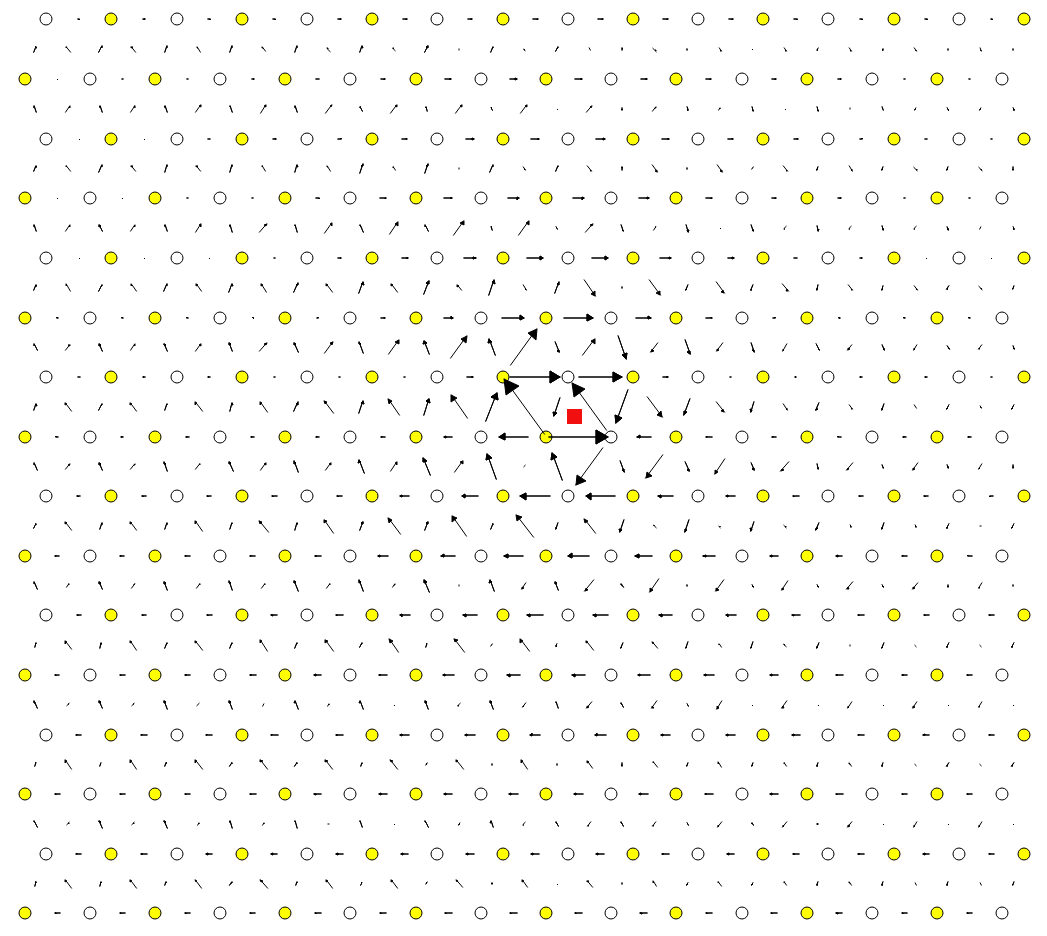
\includegraphics[width=0.5\textwidth]{Images/final_model_IP1_partial_dd_initial.png}
\end{center}
\begin{center}
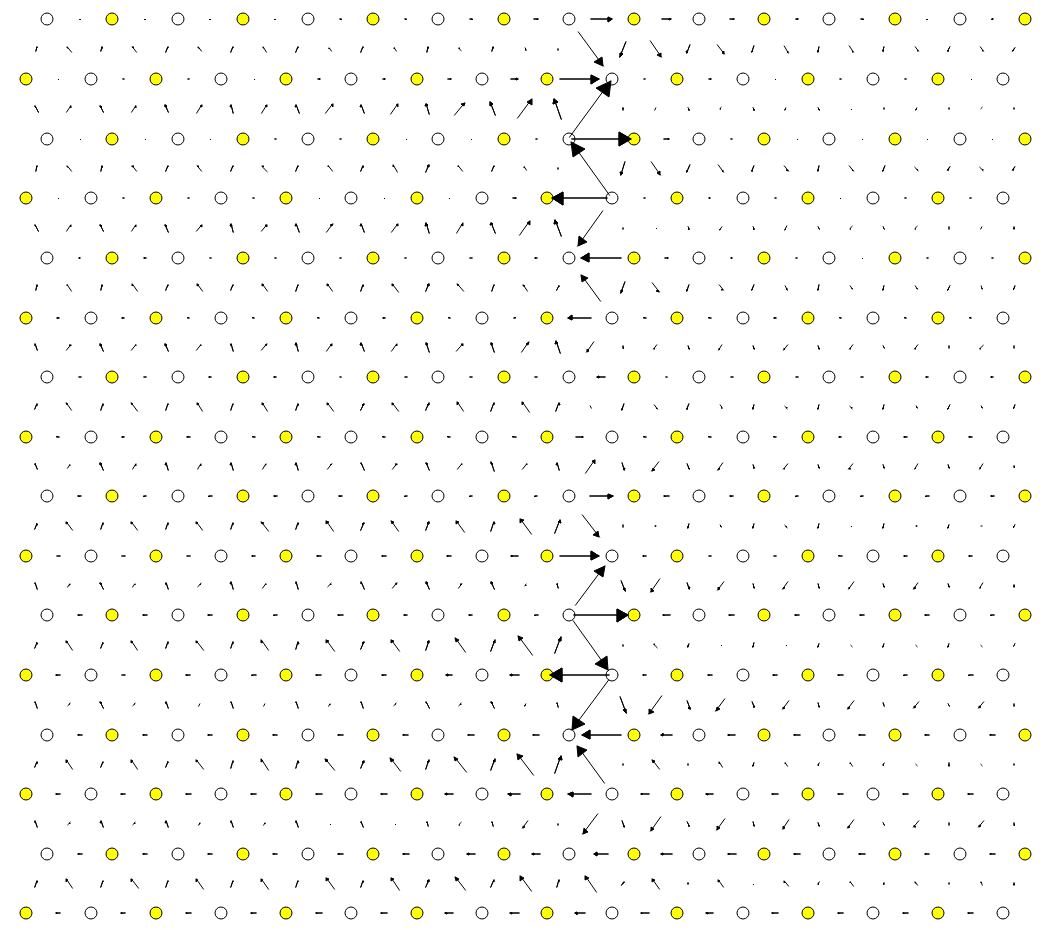
\includegraphics[width=0.5\textwidth]{Images/final_model_IP1_partial_dd_final.png}
\end{center} 

\subsubsection{IP2}
\label{sec:org7b261b4}
\begin{center}
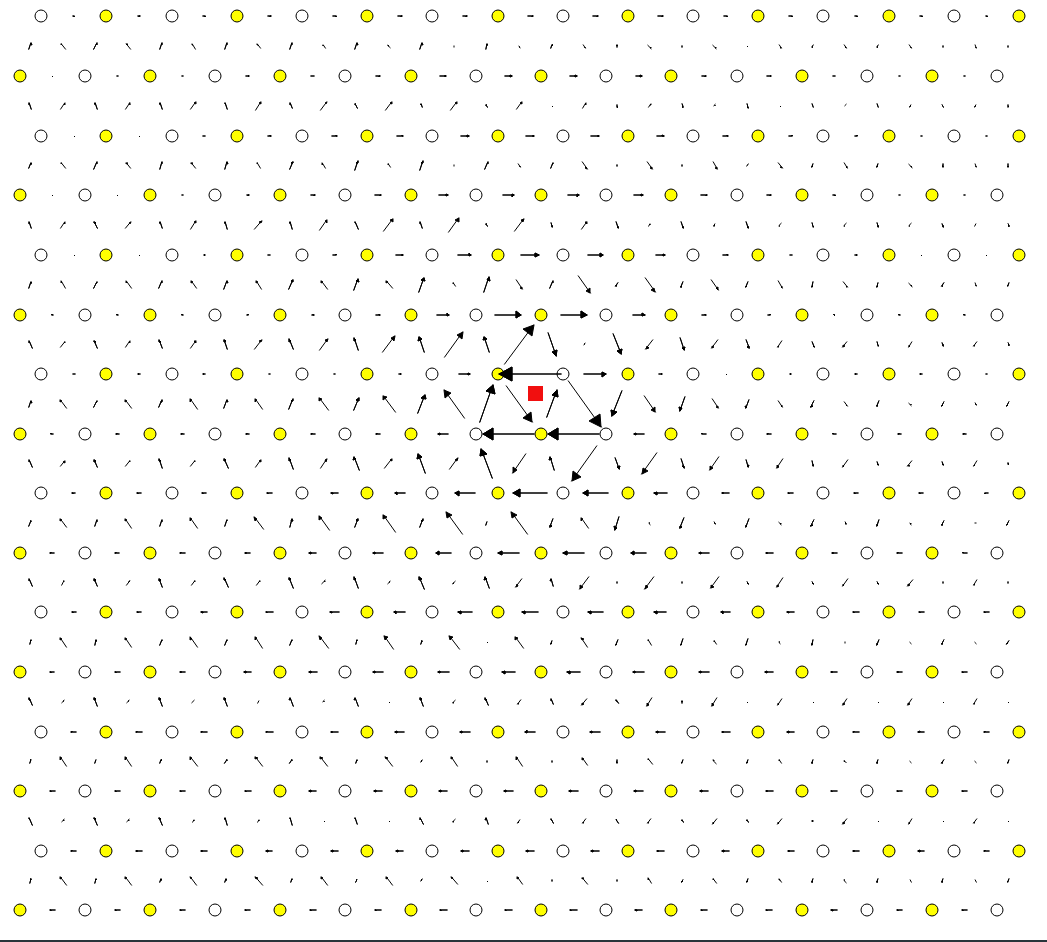
\includegraphics[width=0.5\textwidth]{Images/final_model_IP2_partial_dd_initial..png}
\end{center}
\begin{center}
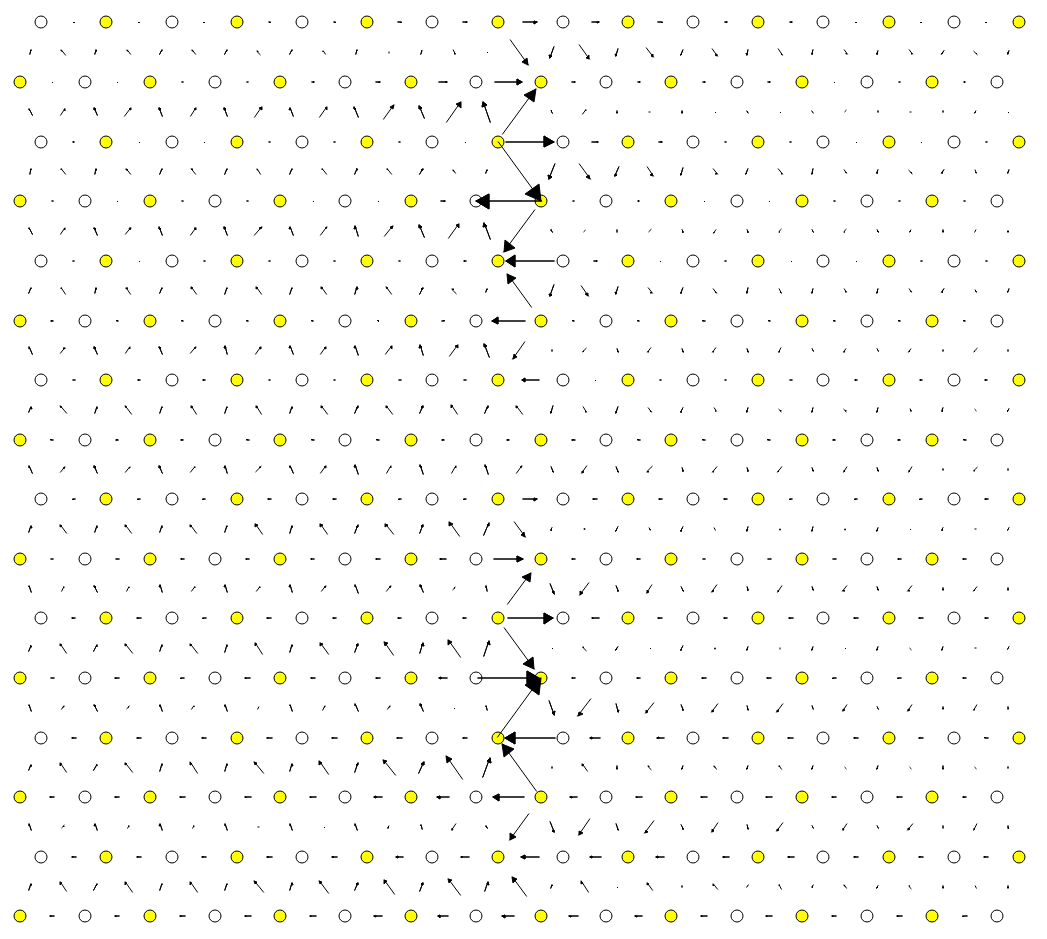
\includegraphics[width=0.5\textwidth]{Images/final_model_IP2_partial_dd_final.png}
\end{center}
\subsubsection{IP3}
\label{sec:org46626d9}
\begin{center}
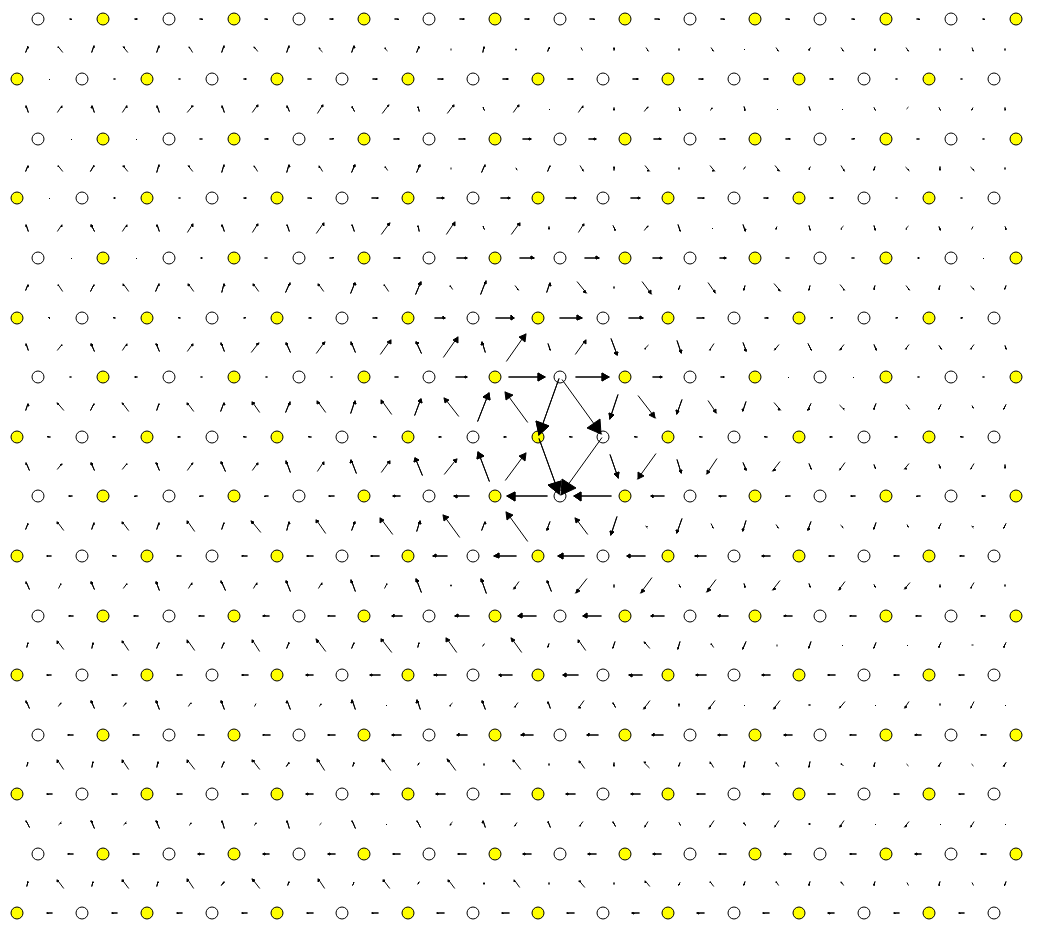
\includegraphics[width=0.5\textwidth]{Images/final_model_IP3_partial_dd_initial.png}
\end{center}
\begin{center}
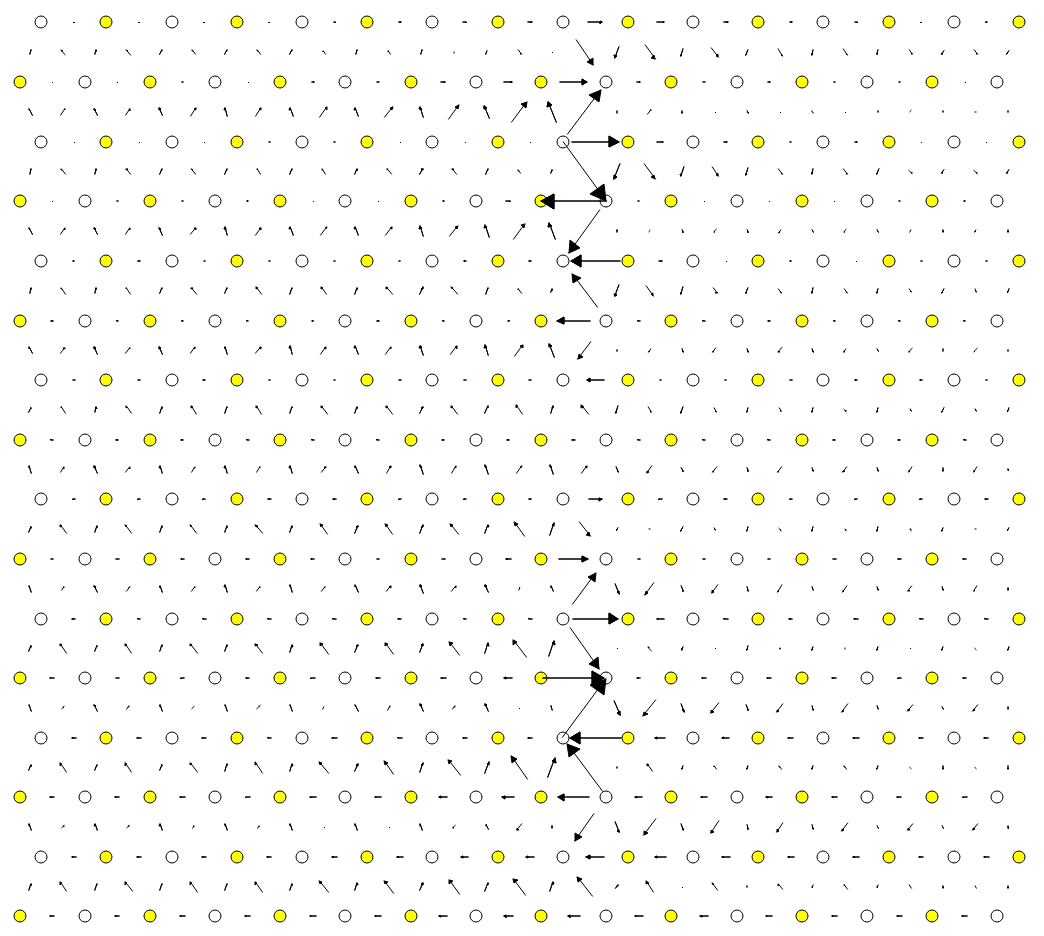
\includegraphics[width=0.5\textwidth]{Images/final_model_IP3_partial_dd_final.png}
\end{center}
\subsubsection{IP4}
\label{sec:orgbd33288}
\begin{center}
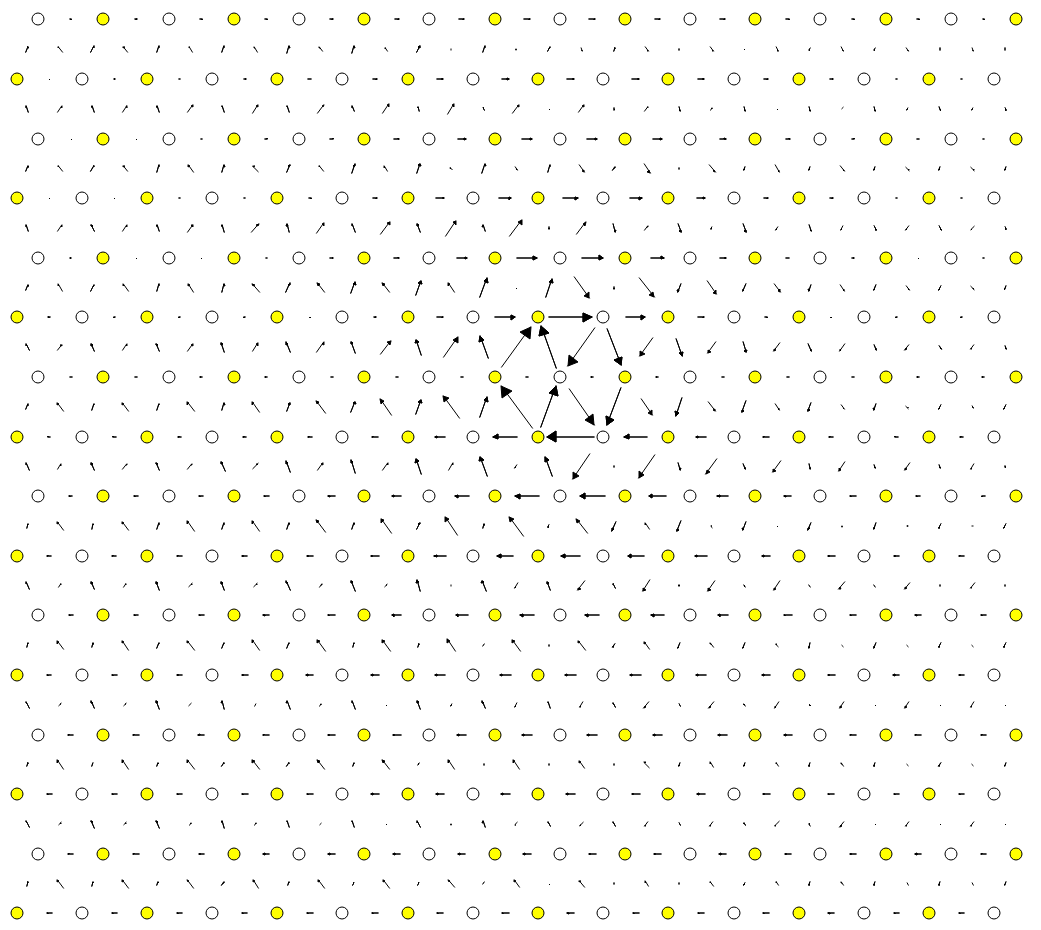
\includegraphics[width=0.5\textwidth]{Images/final_model_IP4_partial_dd_initial.png}
\end{center}
\begin{center}
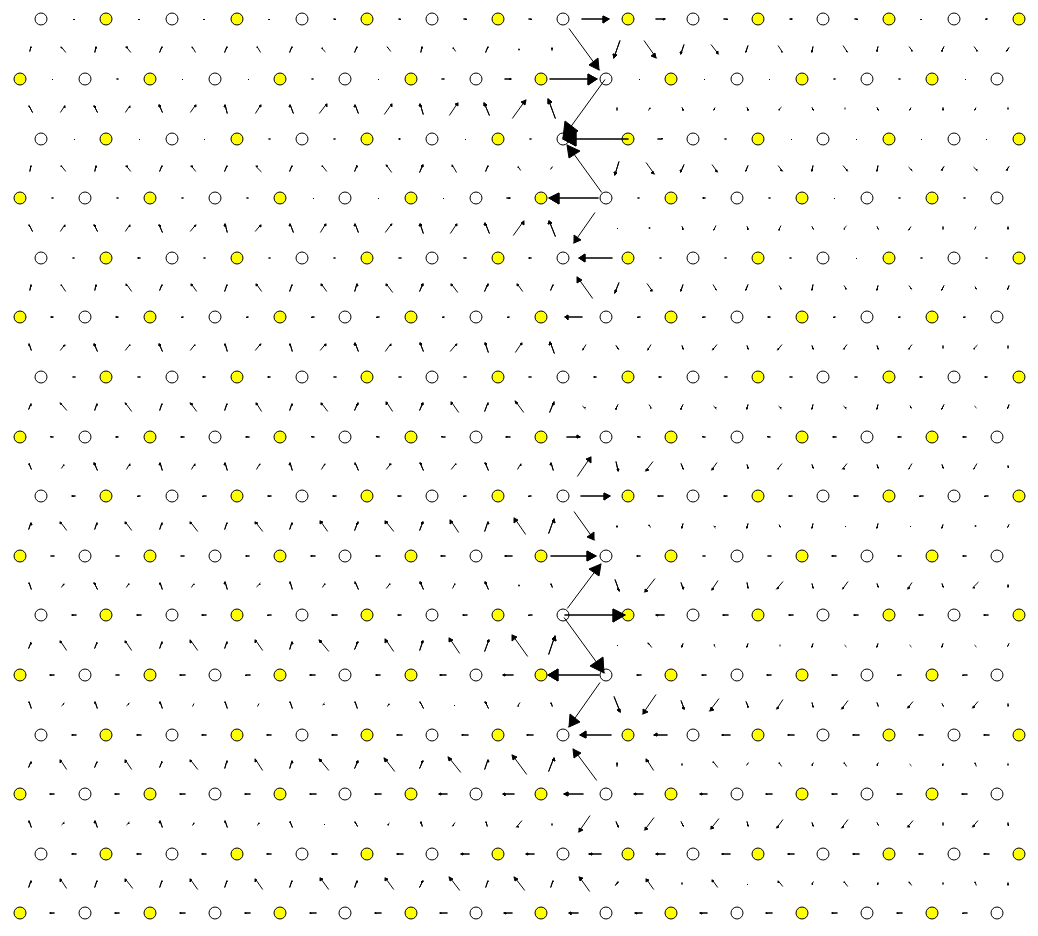
\includegraphics[width=0.5\textwidth]{Images/final_model_IP4_partial_dd_final.png}
\end{center}
\subsubsection{IP5}
\label{sec:org9728f71}
\begin{center}
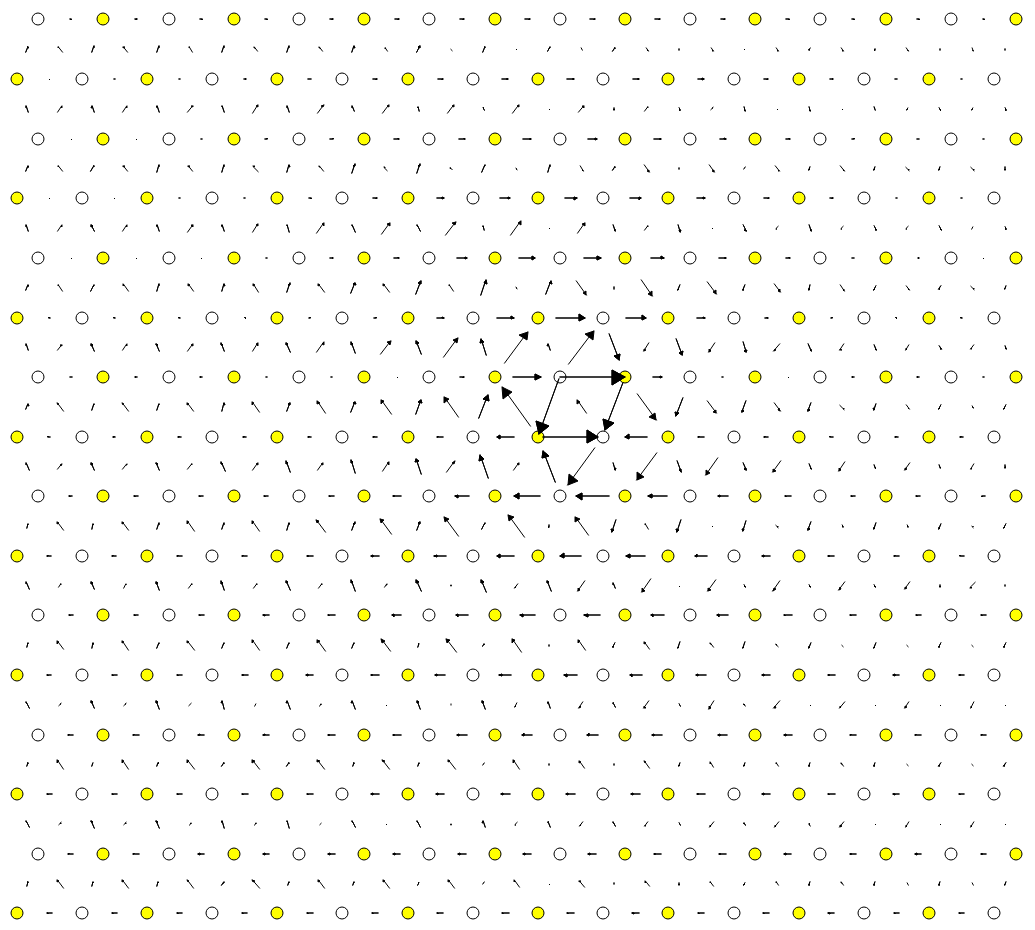
\includegraphics[width=0.5\textwidth]{Images/final_model_IP5_partial_dd_initial.png}
\end{center}
\begin{center}
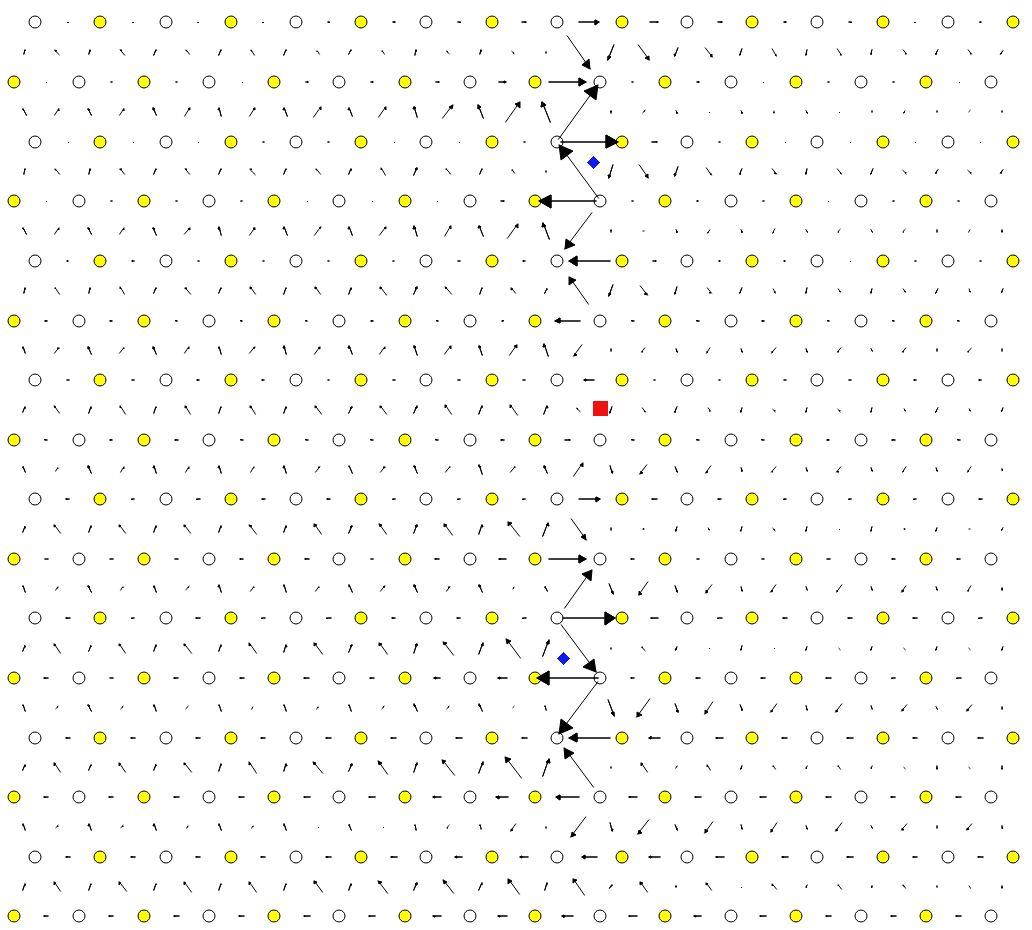
\includegraphics[width=0.5\textwidth]{Images/final_model_IP5_partial_dd_final.png}
\end{center}

\subsubsection{Ghazisaeidi Results for comparison}
\label{sec:orgd12a54f}

\begin{center}
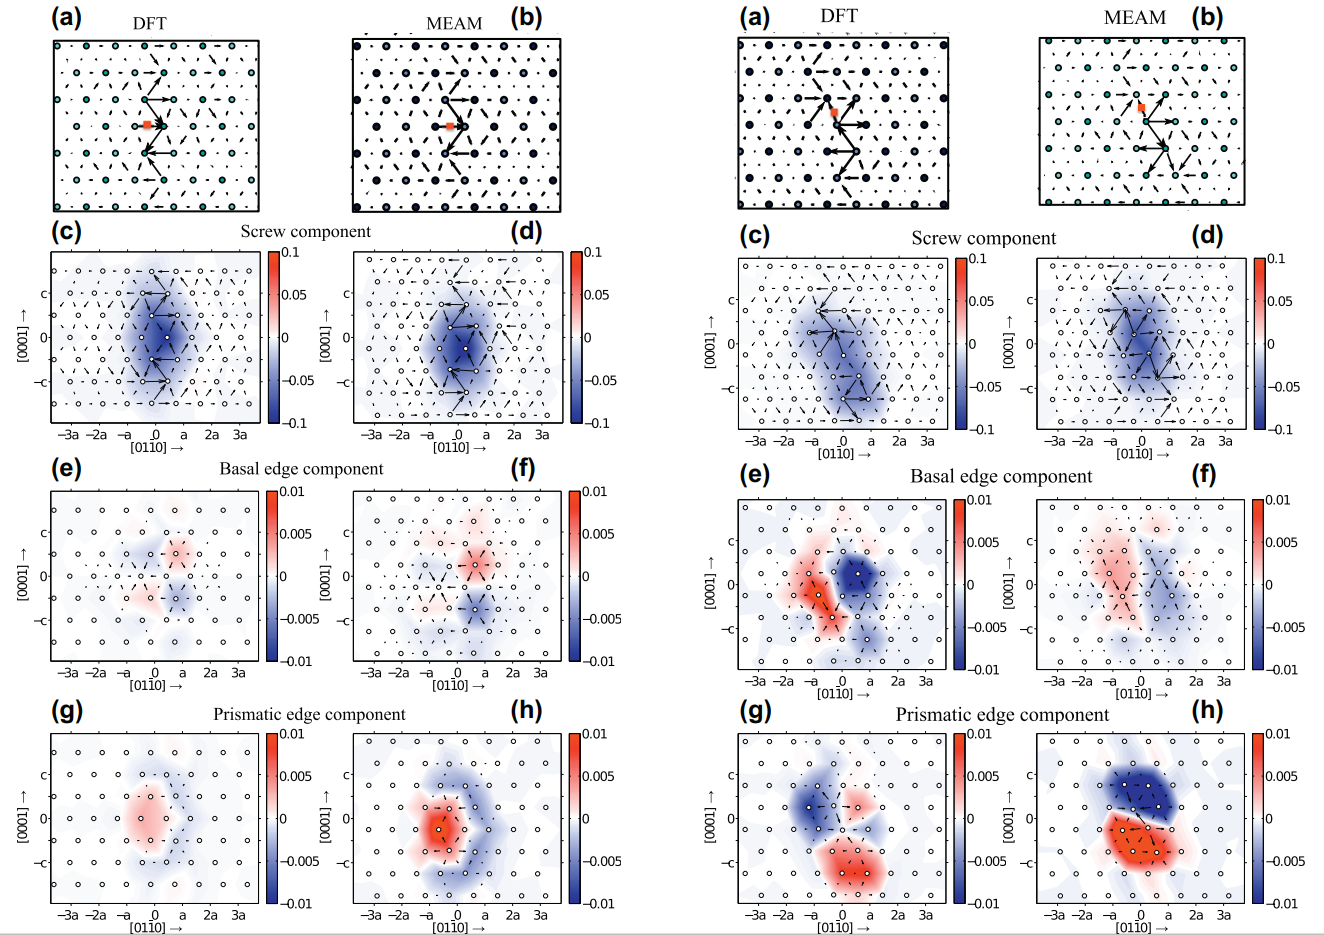
\includegraphics[width=0.5\textwidth]{Images/ghazisaiedi-trinkle-scew-dislocation-core-prism-symm-asymm.png}
\end{center}

\subsubsection{{\bfseries\sffamily TODO} Replot all dislocations and do analysis in Atomman.}
\label{sec:orgb83db0e}
This will be very useful as one can see plots of the Nye tensor, so
one can truly see where the partials are and their dislocation
centres. 

\subsubsection{Peierls Stress}
\label{sec:org182af69}

By straining the cell of a relaxed lattice and incrementally increasing the strain, one
can find the minimum stress necessary to move a dislocation from one
Peierls valley to the next. 

\begin{enumerate}
\item Applying strain
\label{sec:org38476d7}

Applying strain as in \cite{Chen2013}. 

Here we are incrementing the strain by \(0.001C^{\text{rot}}\), where \(C^{\text{rot}}\) is
the transformed elastic constant necessary for transforming a
strain into a stress from the relation \(\sigma_{ij} = C_{ijkl}\varepsilon_{kl}\).

The original elastic constant matrix in its untransformed state
is:

\begin{equation*}
 C =	
  \begin{bmatrix}
   171.6093 &  94.6594 &  61.2262 &   0.     &   0.      &  0.      \\
    94.6594 & 171.6093 &  61.2262 &   0.     &   0.      &  0.      \\
    61.2262 &  61.2262 & 198.9006 &   0.     &   0.      &  0.      \\
     0.     &   0.     &   0.     &  47.4255 &   0.      &  0.      \\
     0.     &   0.     &   0.     &   0.     &  47.4255  &  0.      \\
     0.     &   0.     &   0.     &   0.     &   0.      & 38.4749  
  \end{bmatrix}
\end{equation*}

Transforming it into the dislocation coordinate system, by the
rotation

\begin{equation*}
 R =	
  \begin{bmatrix}
    1 & 0 & 0 \\
    0 & 0 & -1 \\
    0 & 1 & 0 \\
  \end{bmatrix}
\end{equation*}


\begin{equation*}
 C^{\text{rot}}=	
  \begin{bmatrix}
   171.6093 &  61.2262 &  94.6594 &   0.     &   0.      &  0.      \\
    61.2262 & 198.9006 &  61.2262 &   0.     &   0.      &  0.      \\
    94.6594 &  61.2262 & 171.6093 &   0.     &   0.      &  0.      \\
     0.     &   0.     &   0.     &  47.4255 &   0.      &  0.      \\
     0.     &   0.     &   0.     &   0.     &  38.4749  &  0.      \\
     0.     &   0.     &   0.     &   0.     &   0.      & 47.4255  
  \end{bmatrix}
\end{equation*}



For finding the Peierls stress to move partials away from each
other on the prismatic plane plane one finds that the stress if
given by \(\sigma_{xy} = \sigma_{12} =  2C_{66}^{\text{rot}}\varepsilon_{12}\), where \(C_{66}^{\text{rot}} =
     47.4255\) GPa.

To move the whole dislocation on the prismatic plane, one needs a
stress applied which is \(\sigma_xz = \sigma_{13} = 2C_{55}^{\text{rot}}\varepsilon_{13}\), \(C_{55}^{\text{rot}} =
     38.4749\) GPa.

To move the dislocation onto the basal plane one needs to apply as
stress given by \(\sigma_yz = \sigma_{23} = 2C_{44}^{\text{rot}}\varepsilon_{23}\), \(C_{44}^{\text{rot}} =
     47.4255\) GPa.



\item xz Strain
\label{sec:org7b2d34b}

Applying an xz strain to the lattice causes the dislocation to
move along the prismatic plane. 

Using an increment in the strain of \(1\times 10^{-4}C^{*}\), where \(C^{*}\) is
the transformed elastic constant, with a value of \(C_{44}^{*}=38.4749\)
GPa, we find that the dislocation moves from one Peierls
valley along the prismatic plane at \(0.0012C_{44}^{*}\), giving a Peierls
stress of \(\sigma_xz = 2C_{44}\varepsilon_{xz} = 0.0923\) GPa


\begin{center}
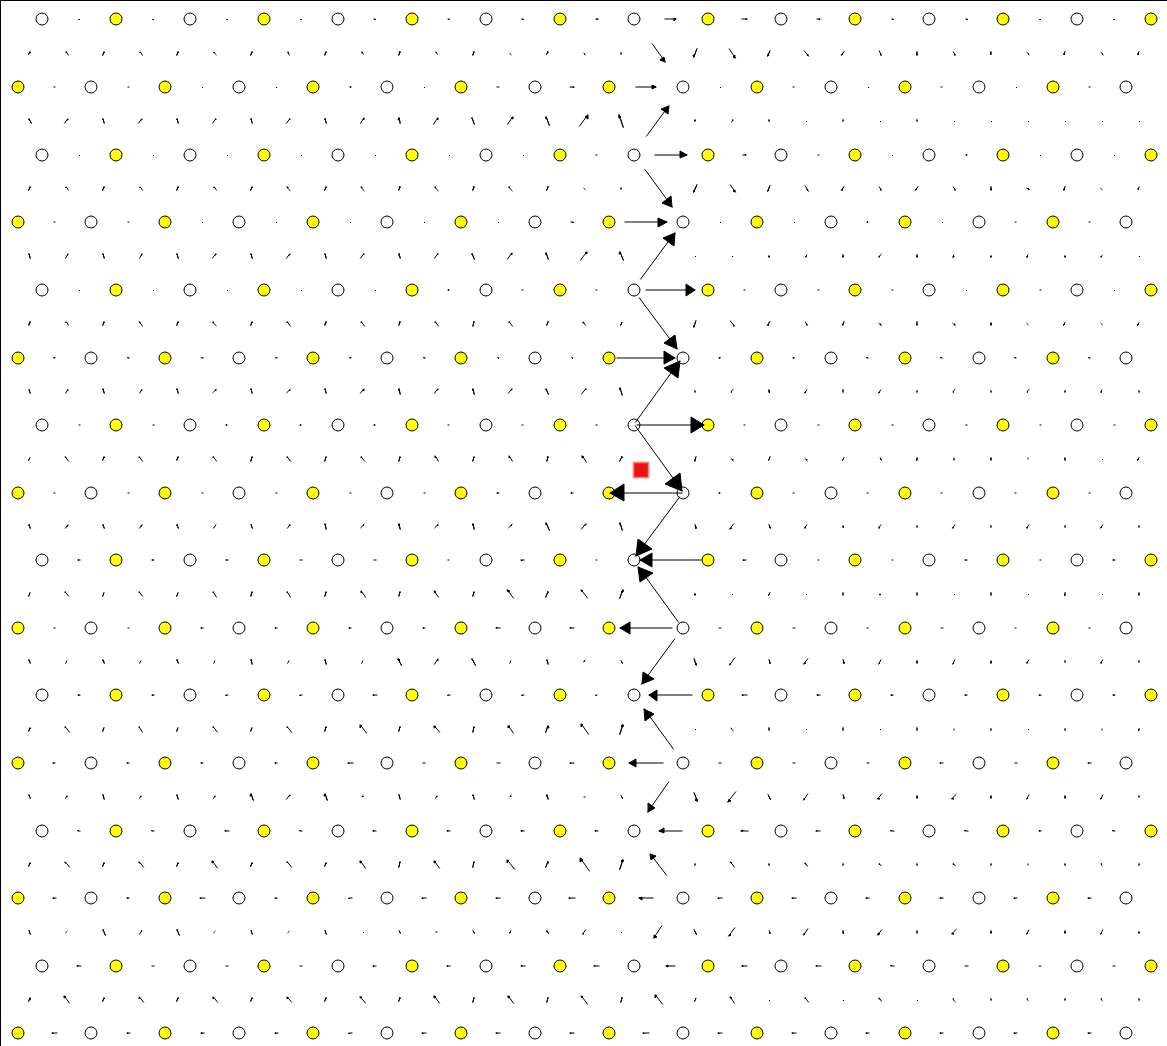
\includegraphics[width=0.5\textwidth]{Images/final_model_peierls_xz_initial.png}
\end{center}
\begin{center}
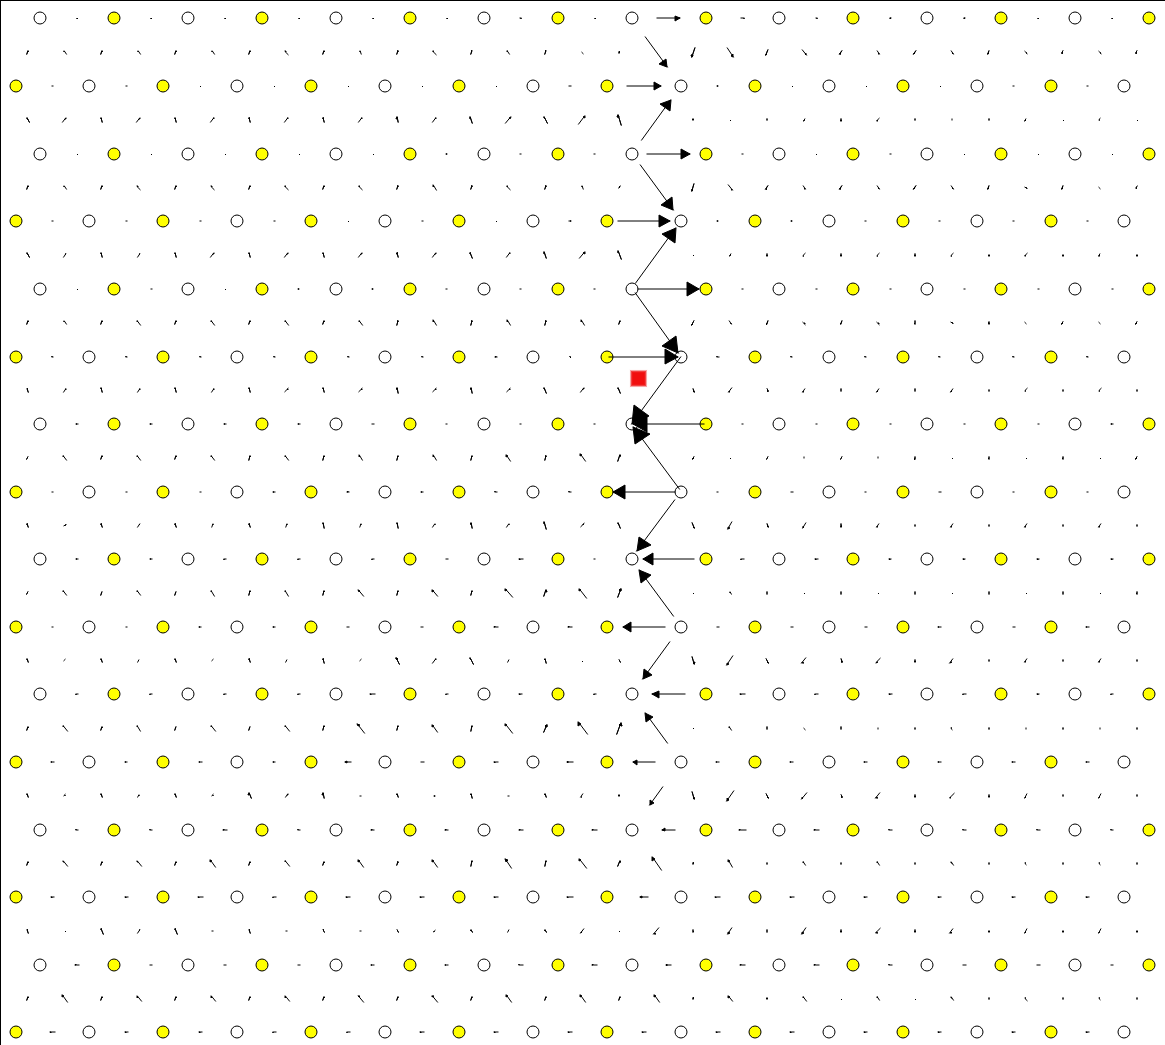
\includegraphics[width=0.5\textwidth]{Images/final_model_peierls_xz_final_0.0012.png}
\end{center}




\item yz Strain
\label{sec:orgbdeeb39}

This is the strain necessary for movement on the basal
plane. Following the procedure above, one does not obtain
recombination of partials, or any movement of the dislocation onto
the basal plane. 

Increasing the accumulated strain up to 10$\backslash$%, still in steps of
0.001C to see if there is any difference. 

Furthermore, one is starting from initial anisotropic elasticity
solutions, applying strain and then relaxing, such that one may be
able to find a strain where the screw dislocation has spread in
the basal plane.


\item xy strain
\label{sec:org1ca1dc6}

An xy strain can move the partials of the prismatic plane apart. 

One can find the Peierls stress for these single partials to move
in opposite directions.

Here the \(\alpha\) parameter is 0.03. 

This means that the stress necessary to move the partial
dislocations apart is 

\begin{align*}
\sigma_{12} &= C_{1212}\varepsilon_{12} \\
    &= 2C^{\text{Voigt}}_{66 }\varepsilon_6^{\text{Voigt}} \\
    &= ( C_{11}- C_{12}) \varepsilon_6^{\text{Voigt}} \\
    &= 47.4255 \times 0.03 \\ 
    &= 1.42 GPa\ 
\end{align*}

The strain is applied to the whole cell, as the dislocation cell
is periodic, then the stress upon each partial is the same. 

\begin{center}
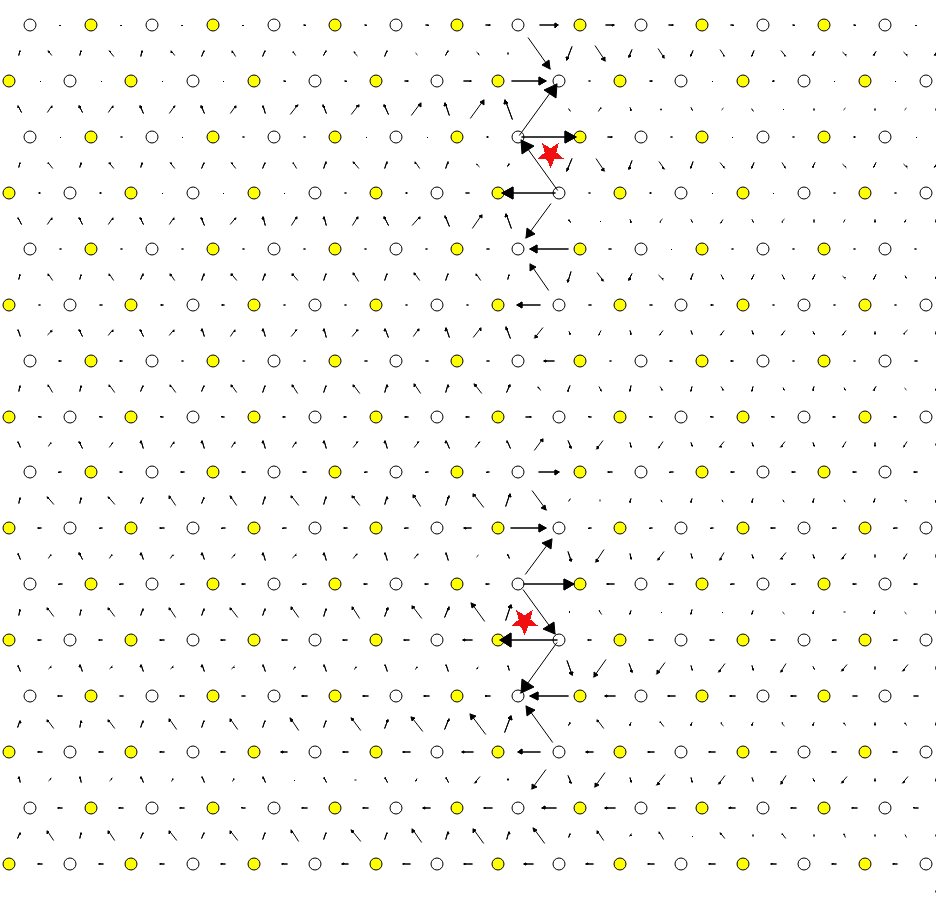
\includegraphics[width=0.5\textwidth]{Images/final_model_peierls_xy_0.03_initial_partials.png}
\end{center}
\begin{center}
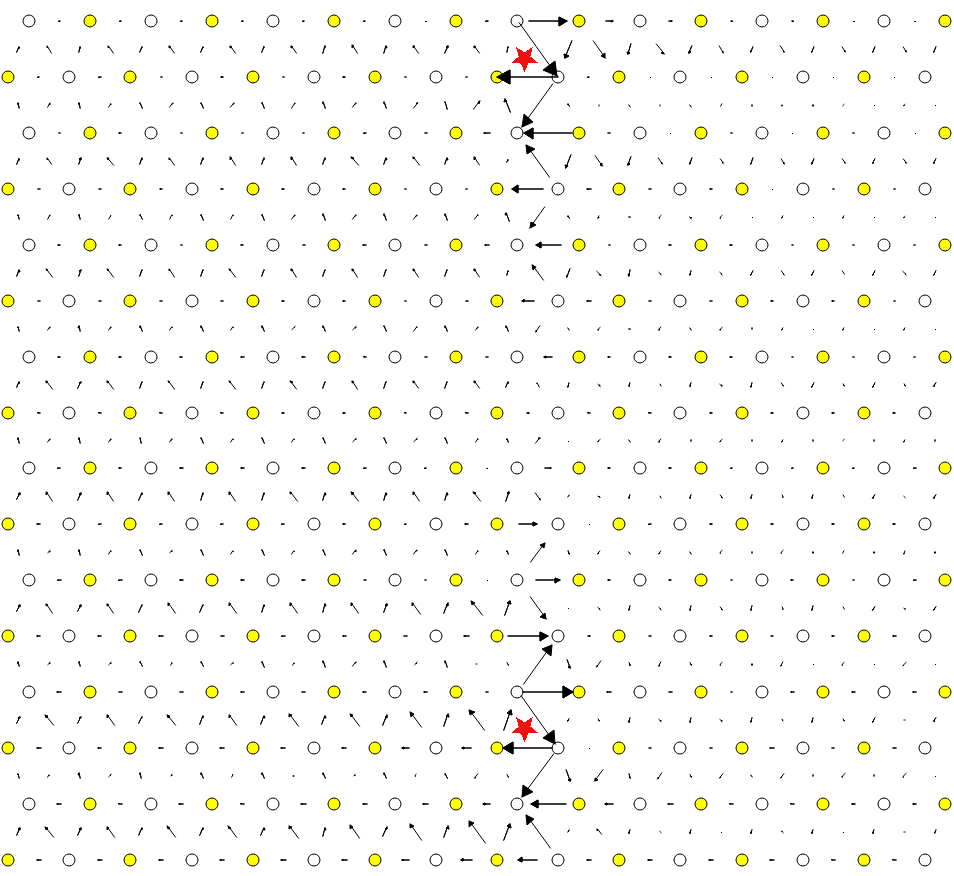
\includegraphics[width=0.5\textwidth]{Images/final_model_peierls_xy_0.03_final_partials.png}
\end{center}


\item Pyramidal Strain
\label{sec:orge9a8c22}

For a strain to transform the dislocation into the metastable,
pyramidal state, one can apply a strain which applies shear to the
dislocation whereby the maximum resolved shear stress is on the
first-order pyramidal plane. 

In the coordinate system of the dislocation, one can estimate the strain necessary by the ratio
of stresses for the basal and prismatic planes. The proportions strains \(\sigma_{xz}\) and
\(\sigma_{yz}\) should be \(c/a : \sqrt{3}/2 \approx 1.83 : 1 \approx 1 : 0.54683\).

Unfortunately, this proportion does not work, nor does the ratio \(\sigma_{xz}:\sigma_{yz}\)
\(\approx\) 1: 1/10\$. A much, much lower proportion of the strain is
necessary as the dislocation just moves prismatically. Once one finds
the Peierls stress for the basal plane, we can estimate a more realistic proportion.
\end{enumerate}


\subsubsection{Data}
\label{sec:orgdd500dc}
\href{file:///home/tigany/Documents/ti/final\_model\_2019-11-12/results\_2019-11-09\_muc/IP1-oo\_19-11-09--04-46-00.log}{IP1}
\href{file:///home/tigany/Documents/ti/final\_model\_2019-11-12/results\_2019-11-09\_muc/IP2-oo\_19-11-09--04-46-00.log}{IP2}
\href{file:///home/tigany/Documents/ti/final\_model\_2019-11-12/results\_2019-11-09\_muc/IP3-oo\_19-11-09--04-46-00.log}{IP3}
\href{file:///home/tigany/Documents/ti/final\_model\_2019-11-12/results\_2019-11-09\_muc/IP4-oo\_19-11-09--04-46-00.log}{IP4}
\href{file:///home/tigany/Documents/ti/final\_model\_2019-11-12/results\_2019-11-09\_muc/IP5-oo\_19-11-09--04-46-00.log}{IP5}

\subsubsection{Directory of the results}
\label{sec:orgde4ca1a}
\url{file:///home/tigany/Documents/ti/2019-09-11\_final\_model/tbe/dislocations/2019-11-08\_no\_omega\_ordering\_ec\_latpar/}
\url{file:///home/tigany/Documents/ti/final\_model\_2019-11}


\subsection{Cluster Method}
\label{sec:org6ce7510}

\subsubsection{Methodology}
\label{sec:org4aaf348}

This secton comprises the results of using the cluster method to
simulate single dislocations in the Ti model. 

The cluster method simulates dislocations by only imposing periodicity in the direction of the
dislocation line (the z-axis, in this case). This the advantage over dislocation dipole
simulations as there are no dislocation-dislocation interactions which interfere with
relaxation, but in their stead, there are dislocation-boundary interactions, which inhibit the
relaxation of the dislocation core.

As the number of atoms in a cluster increases, the resulting core
structure upon relaxation will tend to the bulk core structure, as
there is a reduction in the spurious dislocation-surface
interaction. Due to the finite size of simulations, the geometry
of the cell is important. With sufficient cell size, dislocation
core structure should be invariant to the boundary conditions
imposed. To ascertain how sensitive the new Ti model is to
boundary conditions, two different cell geometries were used:
circular and hexagonal. Each of these had two layers of fixed
(inert) atoms around a dynamic central region.

All relaxations were carried out using the Fletcher-Powell
conjugate gradient algorithm with a force twolerance of \(4\times
    10^{-5}\) Ryd/Bohr \(\approx 1\times 10^{-3} \text{eV}/\AA\), with a
k-point mesh of 1x1x30. 

Tarrat \cite{Tarrat2009} deemed that the use of hexagonal cluster
cell geometries were more beneficial to determine the core
structure of dislocations due to a lower total surface energy,
implying a reduction in the magnitude of dislocation-surface
interaction. 


\subsubsection{Circular Cluster}
\label{sec:org020589b}

 \begin{table}	
\begin{tabular}{ccccccc}
    \small  IP1 & IP2 & IP3 & IP4 & IP5 & IP6 \\ \hline
    % \small Before relaxation ($\mathbf{b} = 1/3\langle 1 \bar{2} 1 0 \rangle$) &
\addheight{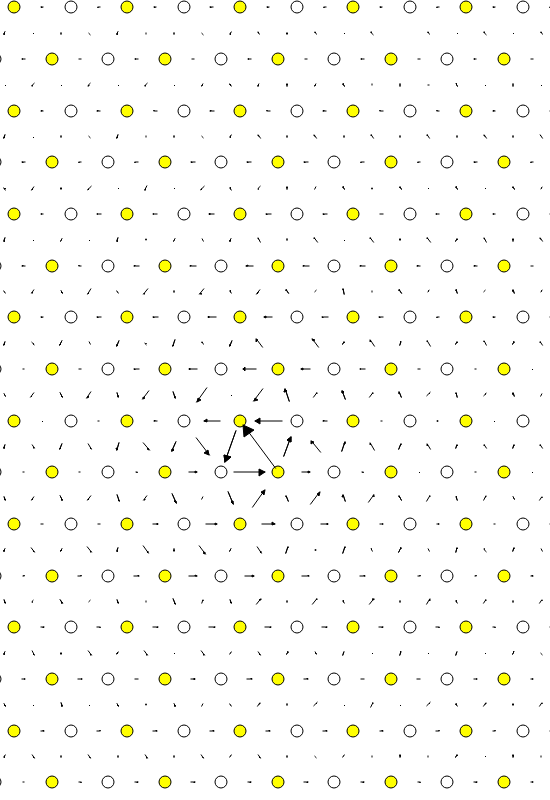
\includegraphics[width=0.165\textwidth]{Images/IP_circle_before_relaxation_full_bvec/crop/IP1_before_full.png}}&
\addheight{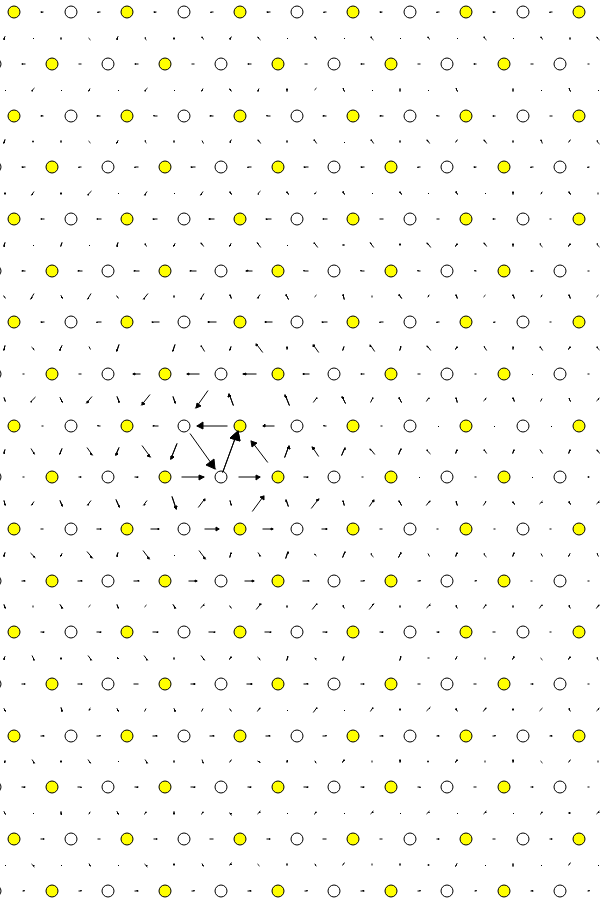
\includegraphics[width=0.165\textwidth]{Images/IP_circle_before_relaxation_full_bvec/crop/IP2_before_full.png}}&
\addheight{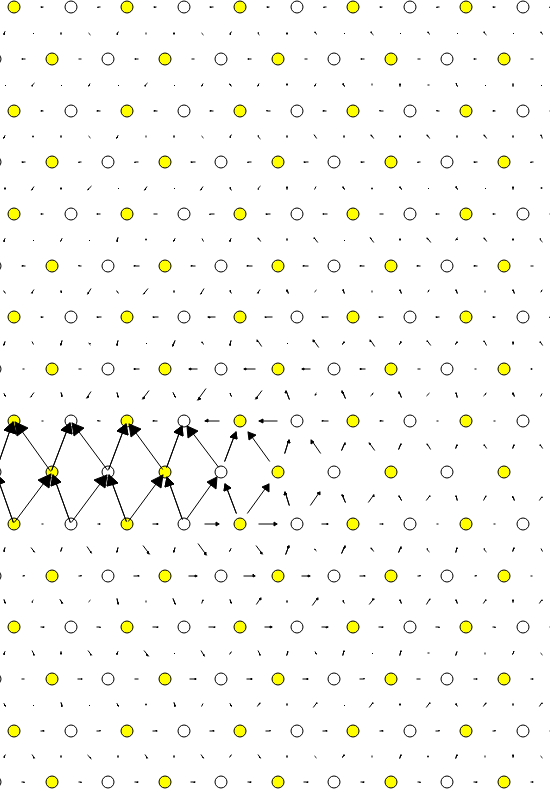
\includegraphics[width=0.165\textwidth]{Images/IP_circle_before_relaxation_full_bvec/crop/IP3_before_full.png}}&
\addheight{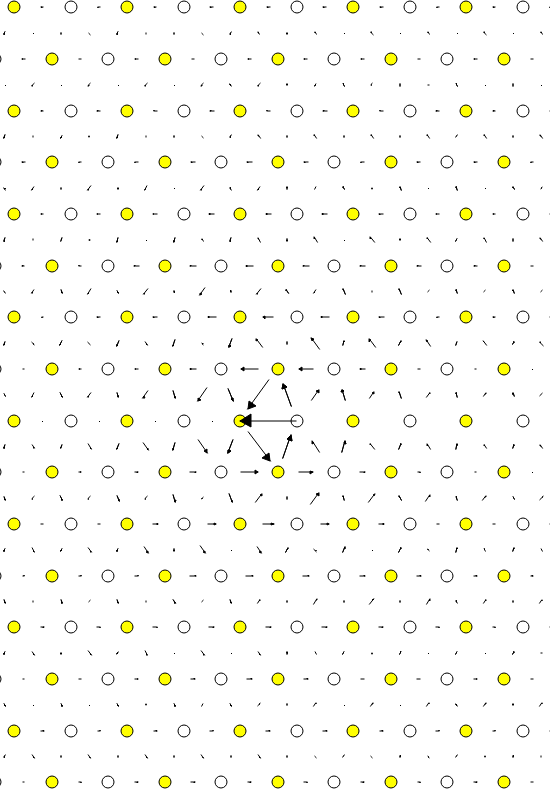
\includegraphics[width=0.165\textwidth]{Images/IP_circle_before_relaxation_full_bvec/crop/IP4_before_full.png}}&
\addheight{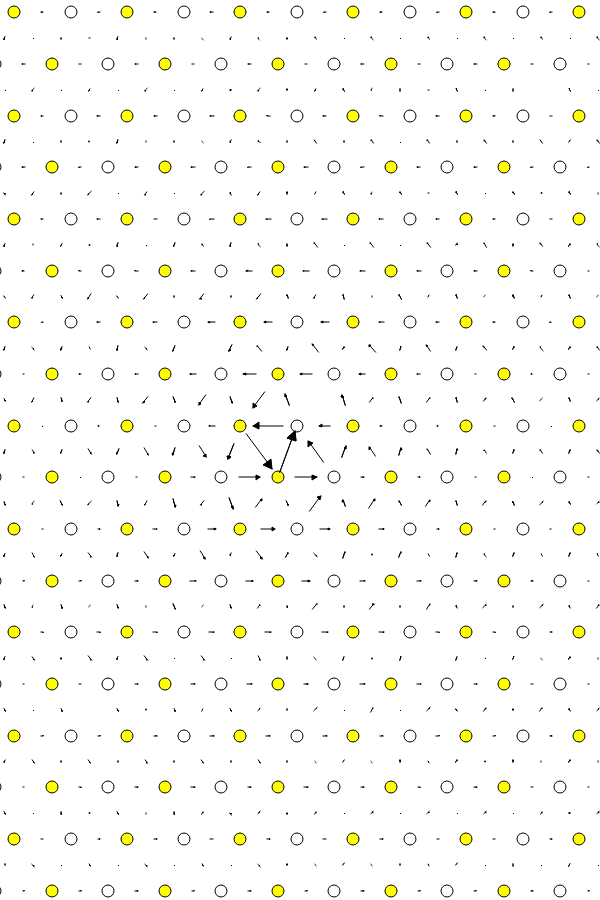
\includegraphics[width=0.165\textwidth]{Images/IP_circle_before_relaxation_full_bvec/crop/IP5_before_full.png}}&
\addheight{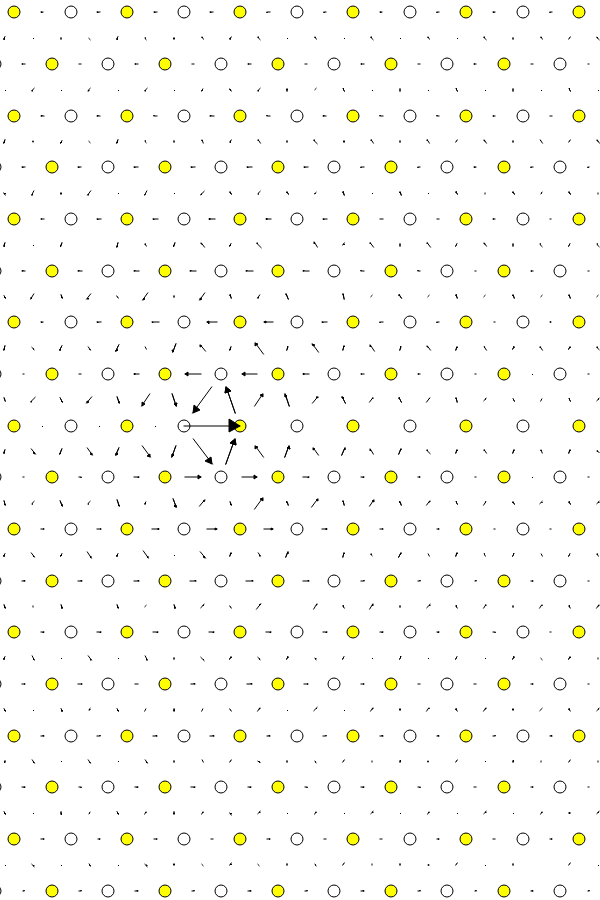
\includegraphics[width=0.165\textwidth]{Images/IP_circle_before_relaxation_full_bvec/crop/IP6_before_full.png}}\\


%	\small After relaxation ($\mathbf{b} = 1/6\langle 1 \bar{2} 1 0 \rangle$) &
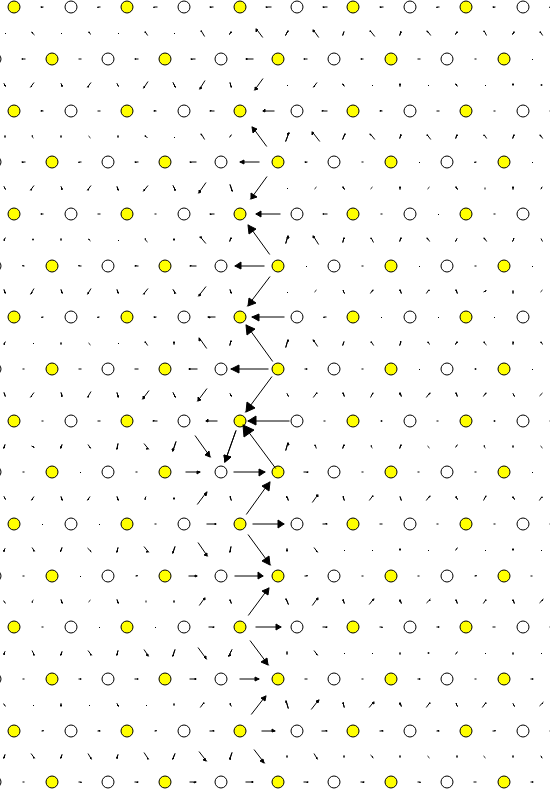
\includegraphics[width=0.165\textwidth]{Images/IP_circle_after_relaxation_full_bvec/crop/IP1_full_initial.png}& 
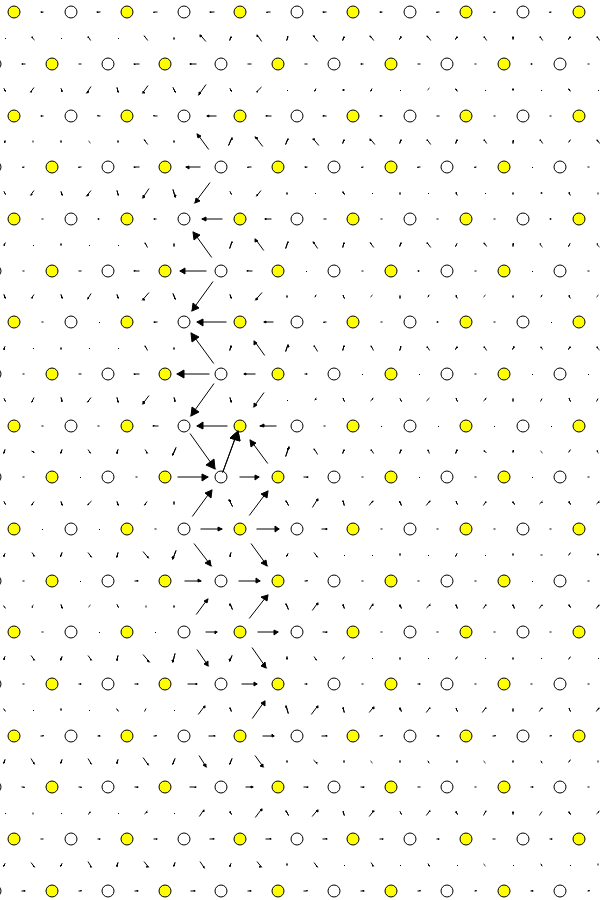
\includegraphics[width=0.165\textwidth]{Images/IP_circle_after_relaxation_full_bvec/crop/IP2_full_initial.png}& 
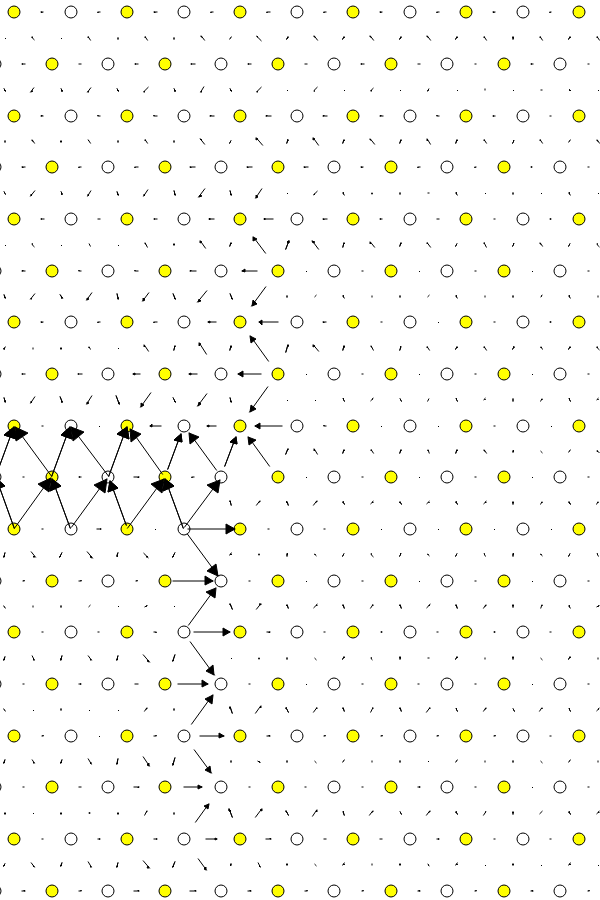
\includegraphics[width=0.165\textwidth]{Images/IP_circle_after_relaxation_full_bvec/crop/IP3_full_initial.png}& 
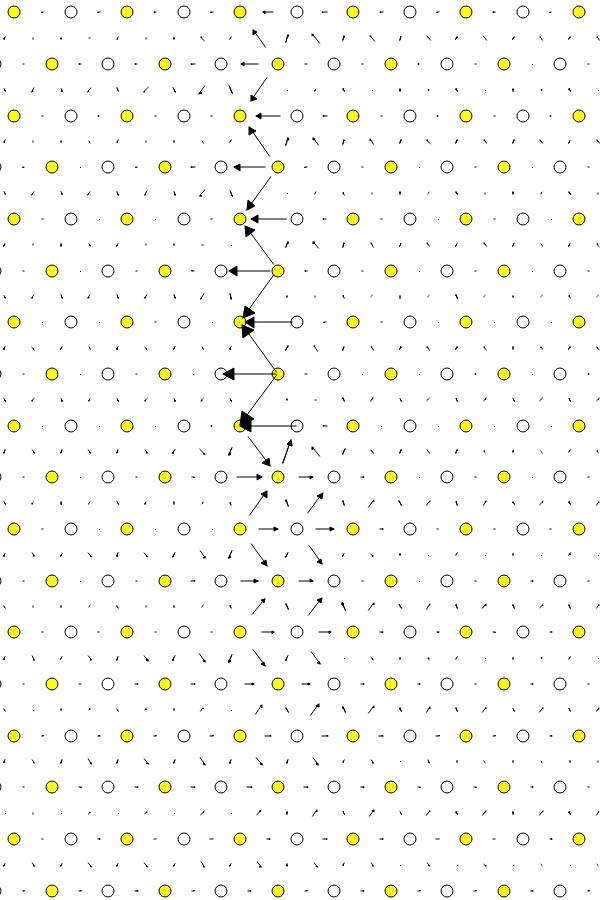
\includegraphics[width=0.165\textwidth]{Images/IP_circle_after_relaxation_full_bvec/crop/IP4_full_initial.png}& 
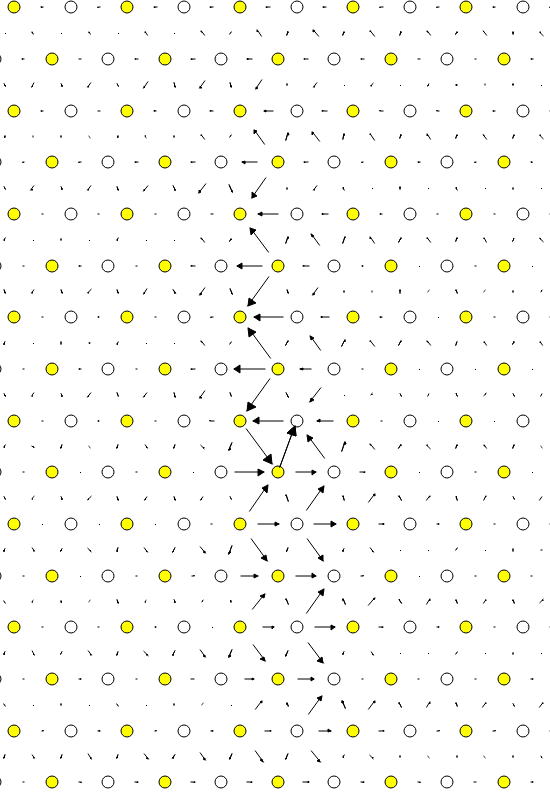
\includegraphics[width=0.165\textwidth]{Images/IP_circle_after_relaxation_full_bvec/crop/IP5_full_initial.png}& 
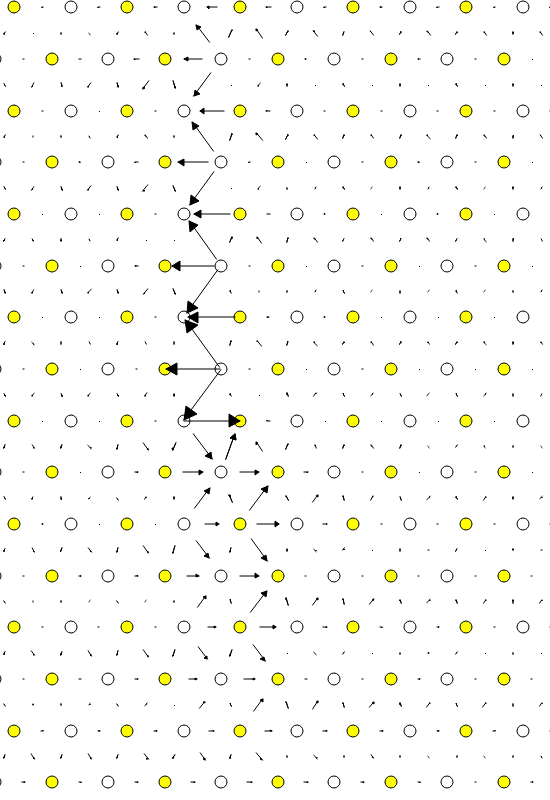
\includegraphics[width=0.165\textwidth]{Images/IP_circle_after_relaxation_full_bvec/crop/IP6_full_initial.png}\\


%	\small After relaxation ($\mathbf{b} = 1/3\langle 1 \bar{2} 1 0 \rangle$) &
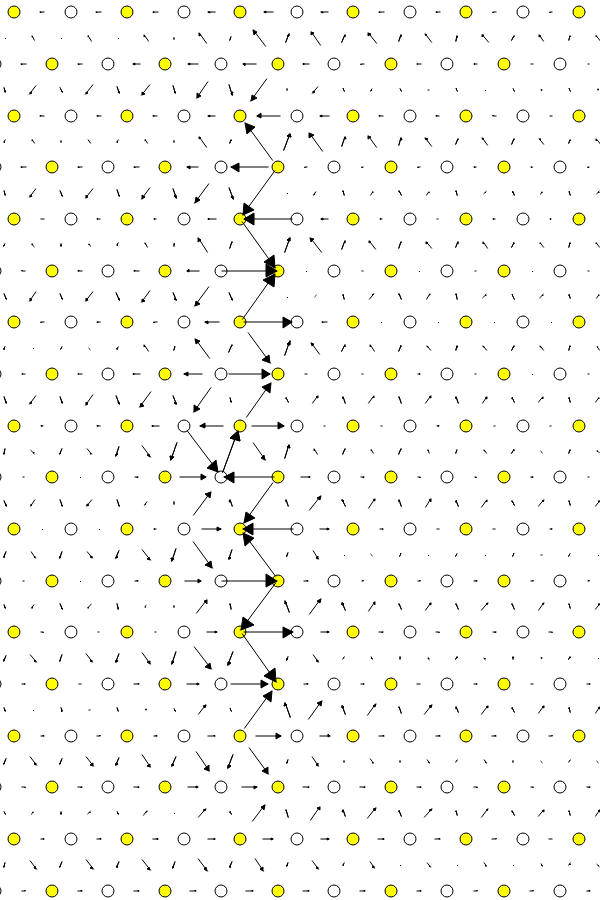
\includegraphics[width=0.165\textwidth]{Images/IP_circle_after_relaxation_half_bvec/crop/IP1_half_relaxed.png}& 
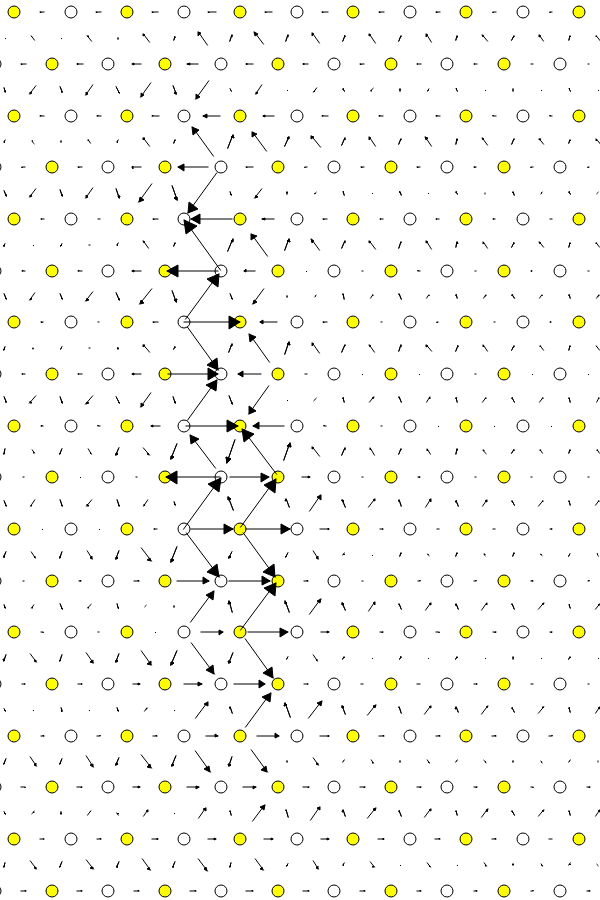
\includegraphics[width=0.165\textwidth]{Images/IP_circle_after_relaxation_half_bvec/crop/IP2_half_relaxed.png}& 
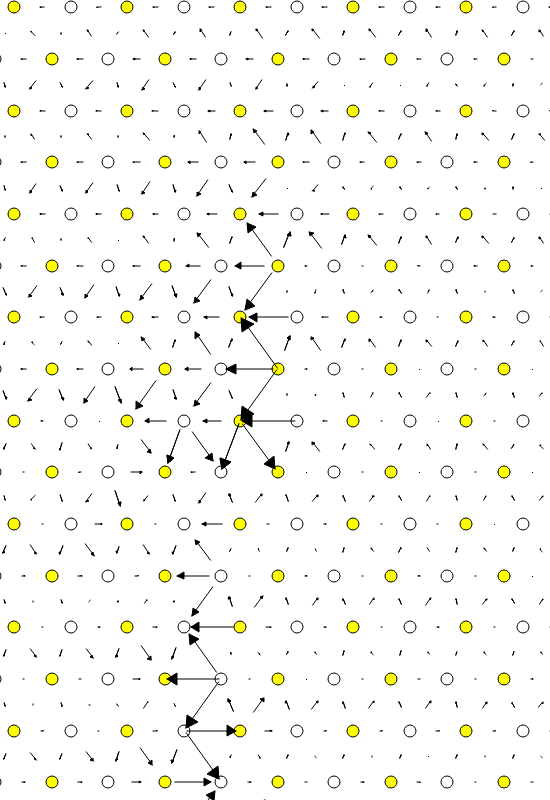
\includegraphics[width=0.165\textwidth]{Images/IP_circle_after_relaxation_half_bvec/crop/IP3_half_relaxed.png}& 
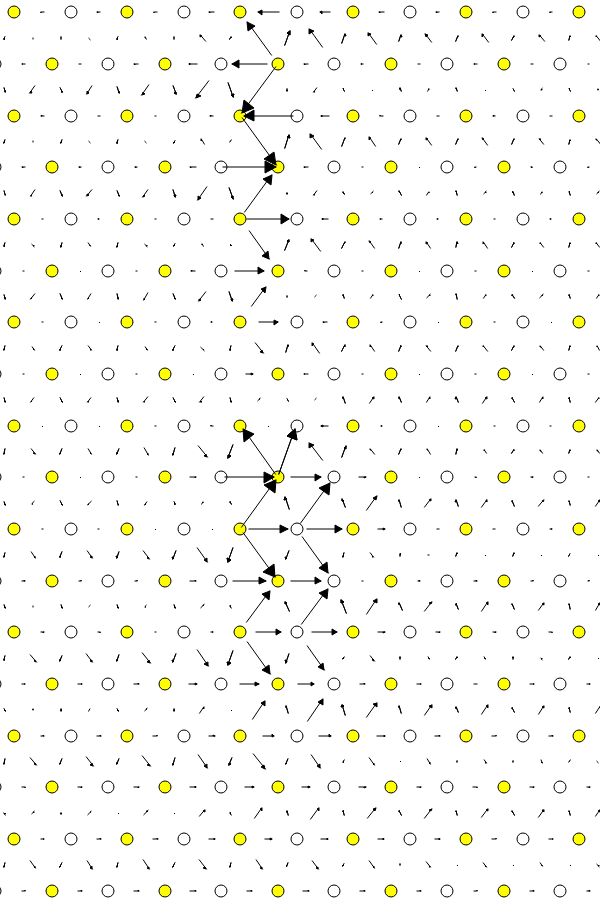
\includegraphics[width=0.165\textwidth]{Images/IP_circle_after_relaxation_half_bvec/crop/IP4_half_relaxed.png}& 
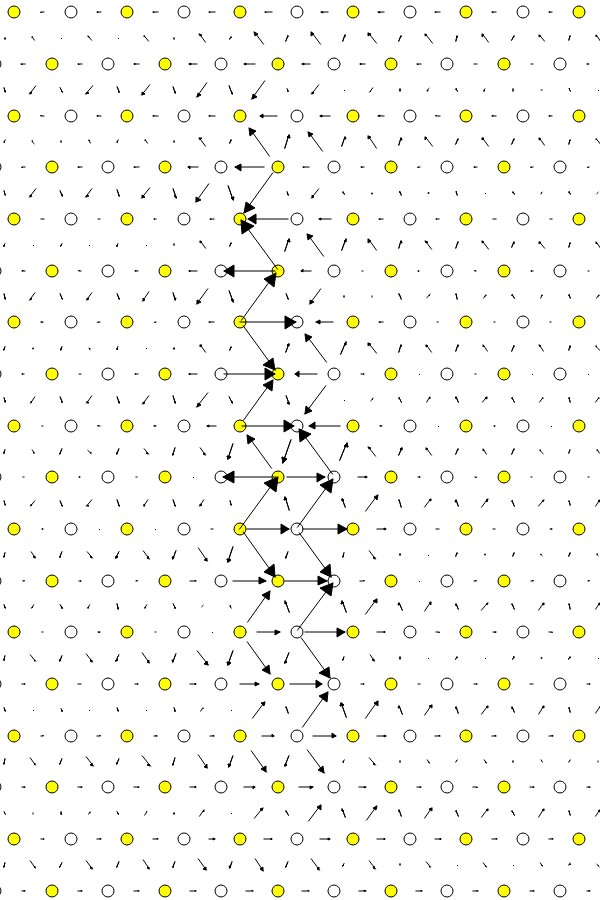
\includegraphics[width=0.165\textwidth]{Images/IP_circle_after_relaxation_half_bvec/crop/IP5_half_relaxed.png}& 
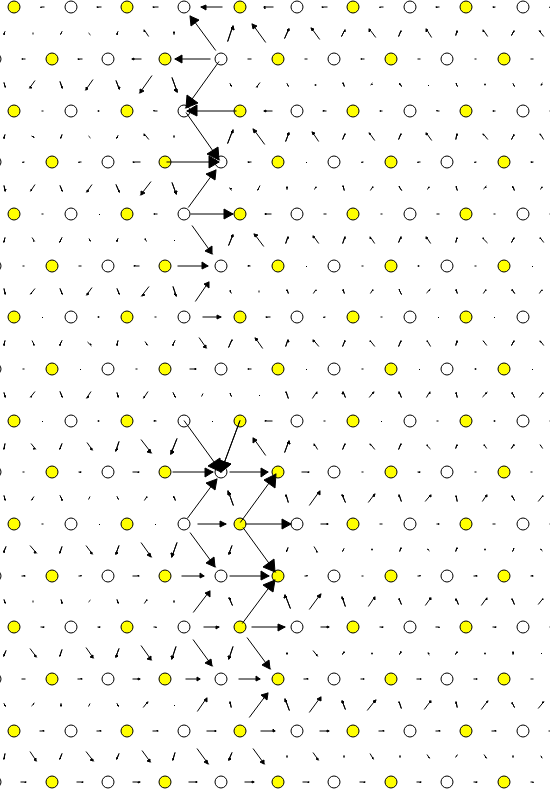
\includegraphics[width=0.165\textwidth]{Images/IP_circle_after_relaxation_half_bvec/crop/IP6_half_relaxed.png}\\

\end{tabular}
\caption{ Differential displacement map of dislocation
relaxations in different initial positions in a cylindrical
cell. Row 1: Prior to relaxation, $\mathbf{b} = 1/3\langle
1\bar{2}10\rangle$. Row 2: After relaxation, $\mathbf{b} = 1/3\langle
1\bar{2}10\rangle$. Row 3: After relaxation, $\mathbf{b} = 1/6\langle
1\bar{2}10\rangle$   }
\end{table}



\subsubsection{Hexagonal Cluster}
\label{sec:org3d60f1a}
\begin{table}
\begin{tabular}{ccccccc}
    \small  IP1 & IP2 & IP3 & IP4 & IP5 & IP6 \\ \hline
    % \small Before relaxation ($\mathbf{b} = 1/3\langle 1 \bar{2} 1 0 \rangle$) &

\addheight{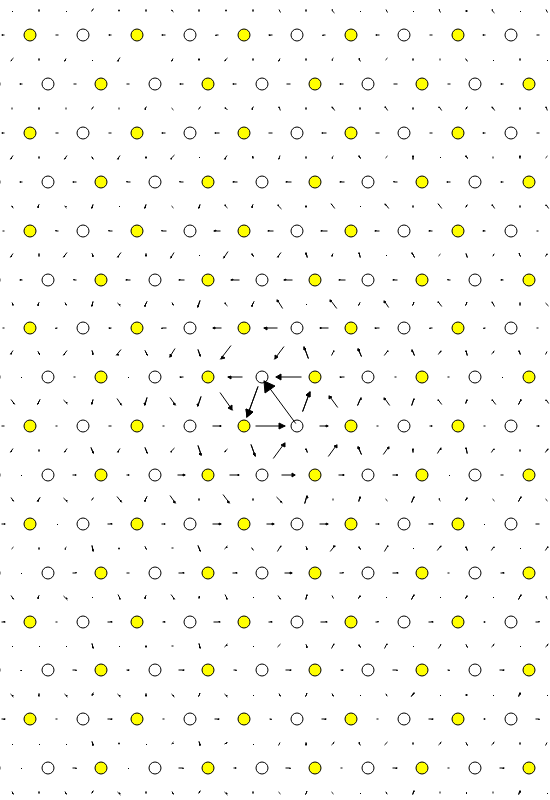
\includegraphics[width=0.165\textwidth]{Images/IP_hex_before_relaxation/crop/IP1_hex_before_full.png}}&
\addheight{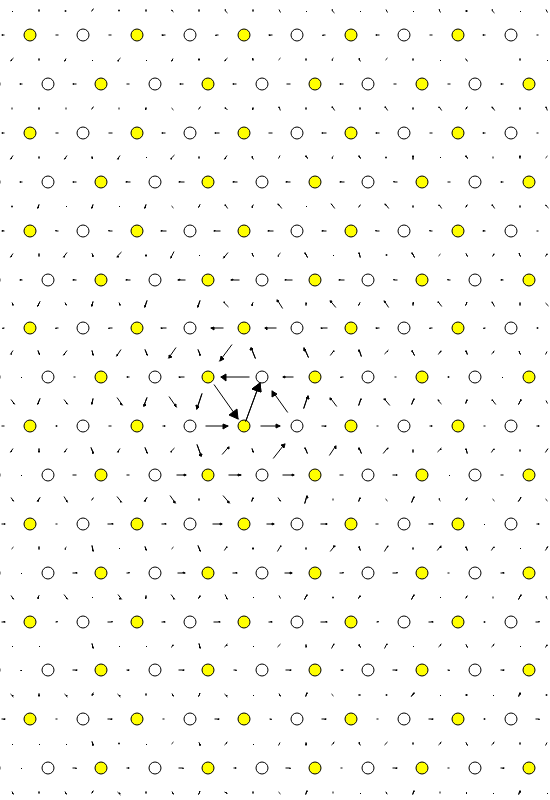
\includegraphics[width=0.165\textwidth]{Images/IP_hex_before_relaxation/crop/IP2_hex_before_full.png}}&
\addheight{\includegraphics[width=0.165\textwidth]{Images/IP_hex_before_relaxation/crop/IP3_hex_before_full.png}}&
\addheight{\includegraphics[width=0.165\textwidth]{Images/IP_hex_before_relaxation/crop/IP4_hex_before_full.png}}&
\addheight{\includegraphics[width=0.165\textwidth]{Images/IP_hex_before_relaxation/crop/IP5_hex_before_full.png}}&
\addheight{\includegraphics[width=0.165\textwidth]{Images/IP_hex_before_relaxation/crop/IP6_hex_before_full.png}}\\


%	\small After relaxation ($\mathbf{b} = 1/6\langle 1 \bar{2} 1 0 \rangle$) &
\includegraphics[width=0.165\textwidth]{Images/IP_hex_after_relaxation_full/crop/IP1_hex_after_relaxation_full.png}& 
\includegraphics[width=0.165\textwidth]{Images/IP_hex_after_relaxation_full/crop/IP2_hex_after_relaxation_full.png}& 
\includegraphics[width=0.165\textwidth]{Images/IP_hex_after_relaxation_full/crop/IP3_hex_after_relaxation_full.png}& 
\includegraphics[width=0.165\textwidth]{Images/IP_hex_after_relaxation_full/crop/IP4_hex_after_relaxation_full.png}& 
\includegraphics[width=0.165\textwidth]{Images/IP_hex_after_relaxation_full/crop/IP5_hex_after_relaxation_full.png}& 
\includegraphics[width=0.165\textwidth]{Images/IP_hex_after_relaxation_full/crop/IP6_hex_after_relaxation_full.png}\\


%	\small After relaxation ($\mathbf{b} = 1/3\langle 1 \bar{2} 1 0 \rangle$) &
\includegraphics[width=0.165\textwidth]{Images/IP_hex_after_relaxation_half/crop/IP1_hex_after_relaxation_half.png}& 
\includegraphics[width=0.165\textwidth]{Images/IP_hex_after_relaxation_half/crop/IP2_hex_after_relaxation_half.png}& 
\includegraphics[width=0.165\textwidth]{Images/IP_hex_after_relaxation_half/crop/IP3_hex_after_relaxation_half.png}& 
\includegraphics[width=0.165\textwidth]{Images/IP_hex_after_relaxation_half/crop/IP4_hex_after_relaxation_half.png}& 
\includegraphics[width=0.165\textwidth]{Images/IP_hex_after_relaxation_half/crop/IP5_hex_after_relaxation_half.png}& 
\includegraphics[width=0.165\textwidth]{Images/IP_hex_after_relaxation_half/crop/IP6_hex_after_relaxation_half.png}\\

\end{tabular}
\caption{ Differential displacement map of dislocation
relaxations in different initial positions in a hexagonal
cell. Row 1: Prior to relaxation, $\mathbf{b} = 1/3\langle
1\bar{2}10\rangle$. Row 2: After relaxation, $\mathbf{b} = 1/3\langle
1\bar{2}10\rangle$. Row 3: After relaxation, $\mathbf{b} = 1/6\langle
1\bar{2}10\rangle$   }
\end{table}



\subsubsection{Peierls Stress}
\label{sec:orgee96a26}

\begin{enumerate}
\item yz strain (basal transformation)
\label{sec:org93d1a7b}

In the cluster method, by incrementally increasing the strain in
increments of 0.001, one found at 0.035 in the IP4 configuration, that
the bottom partial dislocation suddenly splits away from the
prismatic plane the dislocation was spread on.

The dislocations are then of basal character (the partial left on
the prismatic plane being \(1/3\langle 0 \bar{1} 1 0\rangle\), with
the other partial being \(1/3\langle 1 \bar{1} 0 0\rangle\)).

This lower partial moved to the right by 6 lattice parameters and down by
1 clat. There is an I2 (fcc) stacking fault which separates the
prismatic plane from the partial. The core structure is only
basally spread upon movement. 
The other partial moves down the prismatic plane to join the
stacking fault to join in a more compact, yet still basally
dissociated dislocation. The resultant displacements from the
prismatic spreading are removed. 

Then after moving across by 1 alat and up 2 clat, the two
partials stay dissociated on the basal plane, being separated by
4 alat at a maximum. The fcc stacking fault is subsequently
removed by recombination of the dislocations into a compact
\(1/3\langle 1 \bar{2} 1 0 \rangle\) core. This core then begins to
spread in two adjacent prismatic planes with a pyramidal core
spreading joining the two.

The spreading changes from pyramidal with prismatic on two
different prismatic planes, to purely prismatic on the
rightmost prismatic plane. Whereupon, after moving upwards, the
dislocation spreads in this plane identically to the spreading of
an IP4 core configuration upon relaxation.


This means that the Peierls stress for the basal plane, in the
case of a cluster calculation is \(\sigma_{yz} = \sigma_{23} =
     2C_{44}^{\text{rot}}\varepsilon_{23}\), with \(\varepsilon =
     0.035\), and  \(C_{44}^{\text{rot}} = 47.4255\) GPa, we get
\(\sigma_{yz}^{\text{crit.}} = 0.035  \times  47.4255 \approx 1.66\) GPa.


\begin{table}
   \begin{tabular}{ccccc}
      \addheight{\includegraphics[width=0.19\textwidth]{Images/basal_strain_peierls_035/crop/basal_yz_strain_1_cluster.png}}&
      \addheight{\includegraphics[width=0.19\textwidth]{Images/basal_strain_peierls_035/crop/basal_yz_strain_2_cluster.png}}&
      \addheight{\includegraphics[width=0.19\textwidth]{Images/basal_strain_peierls_035/crop/basal_yz_strain_3_cluster.png}}&
      \addheight{\includegraphics[width=0.19\textwidth]{Images/basal_strain_peierls_035/crop/basal_yz_strain_4_cluster.png}}&
      \addheight{\includegraphics[width=0.19\textwidth]{Images/basal_strain_peierls_035/crop/basal_yz_strain_5_cluster.png}}\\

      \includegraphics[width=0.19\textwidth]{Images/basal_strain_peierls_035/crop/basal_yz_strain_6_cluster.png}& 
      \includegraphics[width=0.19\textwidth]{Images/basal_strain_peierls_035/crop/basal_yz_strain_7_cluster.png}& 
      \includegraphics[width=0.19\textwidth]{Images/basal_strain_peierls_035/crop/basal_yz_strain_8_cluster.png}& 
      \includegraphics[width=0.19\textwidth]{Images/basal_strain_peierls_035/crop/basal_yz_strain_9_cluster.png}& 
      \includegraphics[width=0.19\textwidth]{Images/basal_strain_peierls_035/crop/basal_yz_strain_10_cluster.png}\\

      \includegraphics[width=0.19\textwidth]{Images/basal_strain_peierls_035/crop/basal_yz_strain_11_cluster.png}& 
      \includegraphics[width=0.19\textwidth]{Images/basal_strain_peierls_035/crop/basal_yz_strain_12_cluster.png}& 
      \includegraphics[width=0.19\textwidth]{Images/basal_strain_peierls_035/crop/basal_yz_strain_13_cluster.png}& 
      \includegraphics[width=0.19\textwidth]{Images/basal_strain_peierls_035/crop/basal_yz_strain_14_cluster.png}& 
      \includegraphics[width=0.19\textwidth]{Images/basal_strain_peierls_035/crop/basal_yz_strain_15_cluster.png}\\
   \end{tabular}
   \caption{ Behaviour of $\mathbf{b} = 1/3\langle 1\bar{2}10\rangle$ screw dislocation (lime green dot) under action of yz strain to force movement on basal plane. White-coloured atoms denote defected areas of the lattice due to the spreading of dislocations/residual displacement. Red-coloured atoms denote a local hcp structure. Green-coloured atoms denote local fcc structure. The dislocation starts out dissociated in prismatic plane. $\sigma_{yz} \approx 1.66$ GPa forces a prismatic partial to move on its basal plane. The other basal partial moves down to meet the same basal plane as the partial which has broken away. These partials are separated by an I2 stacking fault (green coloured atoms). The basally dissociated partials recombine to form a $1/3\langle 1\bar{2}10\rangle$ screw , whereupon after briefly having a compact core structure, the core spreads in both the pyramidal and prismatic planes, before stabilising in a purely prismatically spread configuration.  }
\end{table}
\end{enumerate}




\subsubsection{Discussion}
\label{sec:org0d7a9e8}

The boundary conditions of the cell seem to be quite important in determining the core
structure. There are differences between the core structure of some of the initial positions
between the hexagonal and cylindrical cells. 

IP1, IP2 and IP5 dislocation centres result in the same core configuration regardless of
the geometry of the cell. 

\section{Binding of oxygen to dislocations}
\label{sec:org96b7199}

\subsection{Quadrupolar Array}
\label{sec:org0ce5af3}

Using a relaxed \(12\times 12\) slab with an "S" quadrupolar
arrangement of dislocations, of which the elastic centres of each
are in initial position 5, one can repeat this cell three times in
the \$z\$-direction. One can place oxygen in octahedral sites near
the dislocation core in the middle layer at varying distances from
the core. By repeating this, one can ascertain how the binding
energy of oxygen to dislocations changes with distance from the
core. 

One does not expect a lot of interaction from the dislocation core
beyond a few burgers vectors of distance of the solute from the
core, as the core field decays rapidly. Beyone this, one would
expect resulting in a lot of the binding energy to come from the
interaction of the strain fields generated by the oxygen
interstitial deforming an octahedral site and the strain field of
the dislocation itself. 


Oxygen was placed near both cores in the simulation cell, such that
the quadrupolar array was more stable. 

Oxygen in the closest octahedral sites in the same basal plane of
the dislocation, unsurprisingly, produced the most change from the
initial dislocation position. Interestingly, it seems that due to
the distortion of the octahedral site from the interstitial oxygen,
the shear stress field produces is above the Peierls stress
necessary for the dislocation to glide on the prismatic plane. This
results in the quadrupolar cores moving to form an S configuration
of an opposite type. 

\begin{center}
\begin{tabular}{rrrr}
Oct Site & E(disl+O)(Ryd) & E(disl+O)-E\(_{\text{p}}\) (eV) & E\(_{\text{int}}\) (meV) = E(disl+O) - E(O) - E(disl) + E(perf) (meV) (from Chaari 2019)\\
1 & -563.15021498 & -44.968444492620 & -82.674534762389\\
2 & -563.13197951 & -44.720338846189 & 165.431111668357\\
3 & -563.15027173 & -44.969216613955 & -83.446656097070\\
4 & -563.15448656 & -45.026562167524 & -140.792209666334\\
5 & -563.13211494 & -44.722181461032 & 163.588496825081\\
6 & -563.13212731 & -44.722349763075 & 163.420194782614\\
7 & -563.15390587 & -45.018661495492 & -132.891537633978\\
8 & -563.14265589 & -44.865598066897 & 20.171890960566\\
9 & -563.14023761 & -44.832695765906 & 53.074191951468\\
10 & -563.13426045 & -44.751372545522 & 134.397412335697\\
\end{tabular}
\end{center}


 \begin{table}	
\begin{tabular}{ccccc}
    \small $E_{\text{int}}$ meV &O1: -82.6 &O2: +165.4 &O3: -83.4 &O4: -140.7 \\ \hline &
    % \small Before relaxation ($\mathbf{b} = 1/3\langle 1 \bar{2} 1 0 \rangle$) &
\addheight{\includegraphics[width=0.19\textwidth]{Images/Ti_IP1-O_interaction/crop/Ti-O1_initial.png}}&
\addheight{\includegraphics[width=0.19\textwidth]{Images/Ti_IP1-O_interaction/crop/Ti-O2_initial.png}}&
\addheight{\includegraphics[width=0.19\textwidth]{Images/Ti_IP1-O_interaction/crop/Ti-O3_initial.png}}&
\addheight{\includegraphics[width=0.19\textwidth]{Images/Ti_IP1-O_interaction/crop/Ti-O4_initial.png}}\\

&
\addheight{\includegraphics[width=0.19\textwidth]{Images/Ti_IP1-O_interaction/crop/Ti-O1_final.png}}&
\addheight{\includegraphics[width=0.19\textwidth]{Images/Ti_IP1-O_interaction/crop/Ti-O2_final.png}}&
\addheight{\includegraphics[width=0.19\textwidth]{Images/Ti_IP1-O_interaction/crop/Ti-O3_final.png}}&
\addheight{\includegraphics[width=0.19\textwidth]{Images/Ti_IP1-O_interaction/crop/Ti-O4_final.png}}\\ \hhline

    \small $E_{\text{int}}$ meV &O5: +163.5 &O6: +163.4 &O7: -132.8& O8: +20.1 \\ \hline &
\addheight{\includegraphics[width=0.19\textwidth]{Images/Ti_IP1-O_interaction/crop/Ti-O5_initial.png}}&
\addheight{\includegraphics[width=0.19\textwidth]{Images/Ti_IP1-O_interaction/crop/Ti-O6_initial.png}}&
\addheight{\includegraphics[width=0.19\textwidth]{Images/Ti_IP1-O_interaction/crop/Ti-O7_initial.png}}&
\addheight{\includegraphics[width=0.19\textwidth]{Images/Ti_IP1-O_interaction/crop/Ti-O8_initial.png}}\\

&
\addheight{\includegraphics[width=0.19\textwidth]{Images/Ti_IP1-O_interaction/crop/Ti-O5_final.png}}&
\addheight{\includegraphics[width=0.19\textwidth]{Images/Ti_IP1-O_interaction/crop/Ti-O6_final.png}}&
\addheight{\includegraphics[width=0.19\textwidth]{Images/Ti_IP1-O_interaction/crop/Ti-O7_final.png}}&
\addheight{\includegraphics[width=0.19\textwidth]{Images/Ti_IP1-O_interaction/crop/Ti-O8_final.png}}\\



\end{tabular}
\caption{ Change in IP1 core structure and dislocation position upon addition of interstitial oxygen in different octahedral sites in a quadrupolar simulation. Row 1: Prior to relaxation. Row 2: After relaxation.   }
\end{table}


\subsection{Notes}
\label{sec:orgc97cded}

A strategy to find the binding energies of different interstitial
sites. 

\begin{enumerate}
\item Find cores of the dislocation using my in-house differential
displacement map analysis.
\item Identify octahedral sites near the cores.
\item Translate octahedral sites from the perfect lattice to the
lattice with a dislocation by the average displacement of the six
surrounding lattice sites.
\item Put the solute into a given interstitial site such that upon
application of the transformation of lattice from one
dislocation core to another (upon rotation and reflection), the
interstitial is in an equivalent position. (If one were to look
at each dislocation in with the burgers vector pointing into the
page, the site should be equivalent.)
\item Relax and find the binding energy by calculating the difference
in energy from the relaxed dislocation to the unrelaxed.
\end{enumerate}


\subsection{Dissolution Energy Equation}
\label{sec:org80e55c0}

The binding energy of oxygen to a dislocation can be given by the
following equation:

\[ E^{\text{sol}}_{\text{O-disl.}} = E_{\text{disl} + n\text{O}} -
   E_{\text{disl}} - \frac{n}{2} E_{\text{O}_2}   \]

Here, the energy of molecular oxygen \(E_{\text{O}_2}/2\) is -5.6eV/atom
from Aksyonov 2016 \cite{Aksyonov2016}. 



\subsection{Current status of simulation}
\label{sec:org8be369a}

An S-arrangement of dislocation dipoles what created in a 12x12
supercell of 576 atoms oriented such that the \(1/3[11\bar{2}0]\)
direction was parallel to the z axis. The dislocation cores were in
the initial position 5 (IP5) and relaxed.

The cell was augmented by two extra periodic images in the
z-direction, creating a 12x12x3 cell of 1728 atoms. 

Oxygen was put into octahedral sites in increasing distance
from each of the cores. The distance was up to four octahedral sites
from the core along the prismatic plane and four prismatic planes
along. This gives 16 sites from which one can extract the
dependence of the dislocation binding energy with distance from the
dislocation core.

These will provide references for the embedding calculations. It is
hoped that embedding will give more accurate answers due to:
\begin{enumerate}
\item There only being one dislocation in an embedding cell:
\begin{itemize}
\item Dislocation strain fields are long-ranged, therefore one can
expect errors due the the additional dislocation-dislocation
interaction upon relaxation.
\end{itemize}
\end{enumerate}


Unfortunately, it was seen with the addition of oxygen to both
cores that the dipole configuration became unstable. Furthermore,
the effective shear stress applied when an oxygen was near the
dislocation core was enough to cause the dislocation to move on the
prismatic plane. 


\section{Peierls Barriers}
\label{sec:orge6b670c}

One can calculate the Peierls barrier to dislocation motion on
particular planes by preparing two relaxed simulation cells, with
the dislocation cores translated with respect to each other on the
plane of interest. 

Evidence from Clouet \cite{Clouet2015} suggests that such a
dislocation core in this initial position (IP1) can undergo a
locking and unlocking mechanism. A prismatically spread \(\langle
  11\bar{2}0 \rangle\) screw core can glide along the wide prismatic
plane with a low shear stress, due to the small Peierls barrier on
this plane. This glissile core is metastable, allowing for
transformation to the ground state configuration of the dislocation
(as found by DFT) which is a sessile, pyramidally spread core on the
first-order pyramidal plane. This is the "locking" mechanism
(whereas unlocking is the opposite: a sessile pyramidal to glissile
prismatic core transformation). This core can then glide on the
pyramidal plane by transformation into a glissile pyramidally spread
core, which has a much higher Peierls barrier (and excess energy)
than the prismatic glissile core, resulting in an increase in
lattice friction dislocation on the pyramidal plane compared to the
prismatic plane.

To calculate these Peierls barriers, first one considered the
prismatic plane. The relaxed IP1 core is situated in a wide
prismatic plane, which has a lower shear stress for glide activation
than the narrow prismatic plane. The dislocation(s) of one cell were
translated by \(\frac{c}{2}\) in the \(y\) direction with respect to the other
cell and relaxed. 

For the basal plane, one translated the dislocation(s) by
\(\frac{\sqrt{3}a}{2}\) in the \(x\) direction. 

For the pyramidal plane, one translated the dislocation by
\([\frac{\sqrt{3}a}{2}, c]\).




\section{BOP}
\label{sec:org97f3617}

\subsection{4 recursion levels}
\label{sec:org26664f3}

kbT = 0.1

>> Lattice parameters:

> hcp
\begin{center}
\begin{tabular}{ll}
a & 2.901660  \AA{}\\
c & 4.747485  \AA{}\\
etot & -18.342162  eV\\
\end{tabular}
\end{center}

> omega
\begin{center}
\begin{tabular}{ll}
a & 7.917318  \AA{}\\
c & 2.749892 \AA{}\\
etot & -17.458700 eV\\
\end{tabular}
\end{center}

Omega is still not as stable as hcp as expected from model. 


>> Elastic Constants

\begin{center}
\begin{tabular}{lrr}
Quantity & calc. (10\(^{\text{11}}\) Pa) & exp. (10\(^{\text{11}}\) GPa)\\
\hline
C11 & 1.781 & 1.761\\
C12 & 0.738 & 0.868\\
C13 & 0.611 & 0.682\\
C33 & 1.969 & 1.905\\
C44 & 0.285 & 0.508\\
C66 & 0.522 & 0.450\\
K & 1.050 & 1.101\\
R & 0.669 & 0.618\\
H & 0.558 & 0.489\\
\end{tabular}
\end{center}

\section{Bibliography}
\label{sec:orgc82a489}
\label{org2289a11}

\bibliographystyle{unsrt}
\bibliography{bibliography/org-refs}
\end{document}